% Bump'em IBMS handbook. Overleaf: upload this folder as a zip, compiler pdfLaTeX, main document main.tex.
\documentclass[11pt,a4paper]{article}

\usepackage[T1]{fontenc}
\usepackage[utf8]{inputenc}
\usepackage{lmodern}
\usepackage[margin=2.2cm]{geometry}
\usepackage{graphicx}
\usepackage{amsmath}
\usepackage{booktabs}
\usepackage{tabularx}
\usepackage{longtable}
\usepackage{array}
\usepackage[table]{xcolor}
\usepackage{listings}
\usepackage{float}
\usepackage{caption}
\usepackage{tikz}
\usetikzlibrary{arrows.meta,positioning,fit,backgrounds,calc}
\usepackage{url}
\usepackage[hidelinks]{hyperref}

\DeclareUrlCommand\urlfile{\urlstyle{tt}}
\DeclareRobustCommand{\file}[1]{\urlfile{#1}}   % repo paths: \file{docs/API.md}
\newcommand{\cmd}[1]{\texttt{#1}}
\newcommand{\fillin}[1]{\par\noindent\colorbox{yellow!40}{\parbox{\dimexpr\linewidth-2\fboxsep}{\raggedright\textbf{TO FILL IN:} #1}}\par}
\newcommand{\warn}[1]{\par\smallskip\noindent\fcolorbox{red!70!black}{red!6}{\parbox{\dimexpr\linewidth-2\fboxsep-2\fboxrule}{\textbf{Danger.} #1}}\par\smallskip}

\definecolor{wyellow}{HTML}{E8C21A}
\definecolor{wblue}{HTML}{2F6FD1}
\definecolor{wgreen}{HTML}{2E9A3E}
\definecolor{wbrown}{HTML}{7A4A21}
\definecolor{wwhite}{HTML}{BBBBBB}

\lstset{basicstyle=\ttfamily\small, columns=fullflexible, breaklines=true, frame=single,
        framerule=0.3pt, rulecolor=\color{black!30}, backgroundcolor=\color{black!3},
        upquote=true, keepspaces=true}

\setlength{\parindent}{0pt}
\setlength{\parskip}{0.5em}
\renewcommand{\arraystretch}{1.15}

\title{\textbf{Bump'em at IBMS Offenburg}\\[0.3em]
\large Hardware review, cabling and software handbook}
\author{Lorenzo Lucchini}
\date{Status: 14 October 2026}

\begin{document}
\maketitle

\begin{abstract}
\noindent This handbook is for students who will use, repair or change the Bump'em cable-perturbation
system at IBMS Offenburg. It compares the original Stanford design and the 2026 master thesis with what is
actually built in the lab, lists what was bought and why, maps every cable from the power supplies to the
motor and from the control board to each module, and explains the software from the Teensy firmware to the
browser UI. The repositories \file{BumpemServer} and \file{BumpemUI} hold the full details; this document
tells you where to look.
\end{abstract}

\begin{center}
\begin{tabular}{ll}
\textbf{BumpemServer} (firmware, server, docs) & \url{https://github.com/lore95/BumpemServer} \\
\textbf{BumpemUI} (web UI) & \colorbox{yellow!40}{\textbf{TO FILL IN:} URL, not on GitHub yet} \\
\end{tabular}
\end{center}

\tableofcontents
\clearpage

\section{The system in one page}

Bump'em pulls a person through a waist harness with up to four motorised ropes while they walk or run
on the GRAIL treadmill. Each rope comes from one \emph{cable module} (tower). One Teensy~4.1
microcontroller controls all four modules: it reads the rope force of each module and commands the motor
current so that the rope holds a small baseline tension (a few N) and, on command, delivers a short force
pulse (the perturbation, up to about 100--150\,N).

The design comes from the Stanford Biomechatronics Lab (Bump'em, ICRA 2020; build guide in
\file{docs/reference/stanford-bumpem-build-guide.pdf}). It was rebuilt at IBMS for the master thesis of
Palanisamy (2026, \file{docs/thesis/thesis.pdf}, user manual \file{docs/thesis/manual.pdf}). From
September 2026 the hardware was re-checked and partly rewired, and the software was rewritten
(firmware v1, Python server, browser UI). This handbook describes that state.

\subsection{Modules and directions}
Directions are given in Vicon axes, seen from above with the subject facing forward. The angle is the
direction in which the subject is \emph{pulled}.

\begin{table}[H]\centering
\begin{tabular}{llrcccc}
\toprule
Module & Tower & Angle & Enable pin & DAC channel & Force pin & Thesis no. \\
\midrule
A & left  & $+90^\circ$  & 27 & VA & 14 (A0) & 1 \\
B & front & $0^\circ$    & 28 & VB & 15 (A1) & 2 \\
C & right & $-90^\circ$  & 29 & VC & 16 (A2) & 3 \\
D & back  & $180^\circ$  & 30 & VD & 17 (A3) & -- (not in the thesis) \\
\bottomrule
\end{tabular}
\caption{Module letters, directions and Teensy pins (\file{docs/knowledge/hardware.md}).}
\end{table}

A diagonal pull (e.g.\ $135^\circ$, back-left) is split over the two neighbouring ropes as a vector:
at $45^\circ$ between two modules each pulls $1/\sqrt{2}$ of the amplitude.

\subsection{Signal and power chain of one module}

\begin{figure}[H]\centering
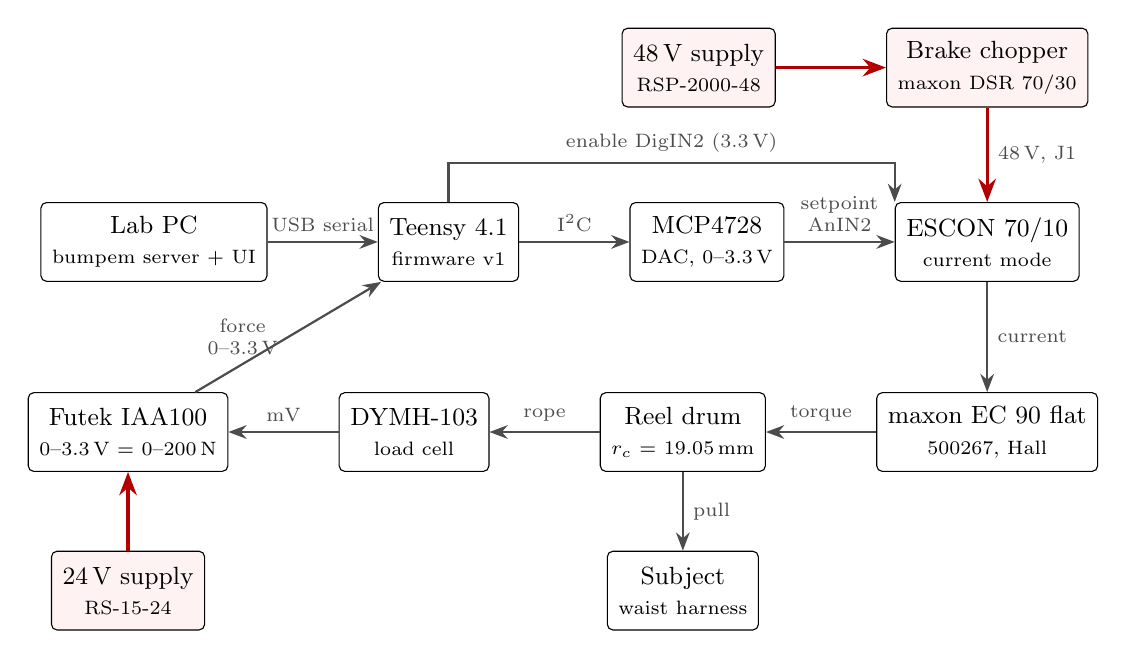
\begin{tikzpicture}[
  box/.style={draw, rounded corners=2pt, align=center, font=\small, minimum height=1.0cm, inner sep=4pt},
  sig/.style={-{Stealth}, thick, black!70},
  pwr/.style={-{Stealth}, very thick, red!70!black},
  lab/.style={font=\scriptsize, black!70, align=center}]
  \node[box] (pc) {Lab PC\\\scriptsize bumpem server + UI};
  \node[box, right=1.4cm of pc] (teensy) {Teensy 4.1\\\scriptsize firmware v1};
  \node[box, right=1.4cm of teensy] (dac) {MCP4728\\\scriptsize DAC, 0--3.3\,V};
  \node[box, right=1.4cm of dac] (escon) {ESCON 70/10\\\scriptsize current mode};
  \node[box, below=1.4cm of escon] (motor) {maxon EC 90 flat\\\scriptsize 500267, Hall};
  \node[box, left=1.4cm of motor] (drum) {Reel drum\\\scriptsize $r_c$ = 19.05\,mm};
  \node[box, left=1.4cm of drum] (cell) {DYMH-103\\\scriptsize load cell};
  \node[box, left=1.4cm of cell] (amp) {Futek IAA100\\\scriptsize 0--3.3\,V = 0--200\,N};
  \node[box, above=1.2cm of escon, fill=red!5] (chop) {Brake chopper\\\scriptsize maxon DSR 70/30};
  \node[box, left=1.4cm of chop, fill=red!5] (psu48) {48\,V supply\\\scriptsize RSP-2000-48};
  \node[box, below=1.0cm of amp, fill=red!5] (psu24) {24\,V supply\\\scriptsize RS-15-24};
  \node[box, below=1.0cm of drum] (subj) {Subject\\\scriptsize waist harness};

  \draw[sig] (pc) -- node[lab, above]{USB serial} (teensy);
  \draw[sig] (teensy) -- node[lab, above]{I$^2$C} (dac);
  \draw[sig] (dac) -- node[lab, above]{setpoint\\AnIN2} (escon);
  \draw[sig] (teensy.north) |- ++(0,0.5) -| node[lab, pos=0.25, above]{enable DigIN2 (3.3\,V)} (escon.north west);
  \draw[sig] (escon) -- node[lab, right]{current} (motor);
  \draw[sig] (motor) -- node[lab, above]{torque} (drum);
  \draw[sig] (drum) -- node[lab, above]{rope} (cell);
  \draw[sig] (cell) -- node[lab, above]{mV} (amp);
  \draw[sig] (amp) -- node[lab, left]{force\\0--3.3\,V} (teensy);
  \draw[sig] (drum) -- node[lab, right]{pull} (subj);
  \draw[pwr] (psu48) -- (chop);
  \draw[pwr] (chop) -- node[lab, right]{48\,V, J1} (escon);
  \draw[pwr] (psu24) -- (amp);
\end{tikzpicture}
\caption{One module. Black: signals; red: power. Teensy, DAC and lab PC are shared by all four modules;
everything else exists once per module.}
\label{fig:chain}
\end{figure}

\subsection{State on 14 October 2026}
\begin{table}[H]\centering
\begin{tabularx}{\linewidth}{lX}
\toprule
Module & State \\
\midrule
A (left)  & Works open loop and closed loop (held 2\,N on 6 Oct). \\
B (front) & Former broken tower. Chopper, motor and new 48\,V supply checked OK. Its ESCON is faulty
            (enable ignored, USB not recognised); replacement ordered 7 Oct, not yet arrived. \\
C (right) & Works open loop. Force reading invalid (about 73\,N at rest) because of a cut ground wire;
            repaired when the cables move to the carrier board. \\
D (back)  & Works open loop and closed loop (held 2\,N on 6 Oct). \\
\midrule
Control board & Teensy and DAC still on a breadboard. Carrier PCB being made by the HS Offenburg
            makerspace (expected 16 Oct). \\
Safety    & Hardware e-stop not wired yet: the power strip switch is the only stop for the motors. \\
Software  & Firmware v1 on the Teensy; server 0.4.0 and UI tested on the simulator and partly on the real board.
            Gait-triggered perturbations (PTO), trials and live Vicon are not built yet. \\
\bottomrule
\end{tabularx}
\caption{Status. The live version is in \file{docs/STATUS.md} and \file{docs/TODO.md}.}
\end{table}

\section{Rebuild from zero}\label{sec:rebuild}
Follow this section in order to go from nothing to the system as it was on 14 October 2026. Each step
ends with a check. Do not go on until it passes. The later sections give the details for each step.

\subsection{What ``the current version'' is}
\begin{table}[H]\centering\small
\begin{tabularx}{\linewidth}{lX}
\toprule
Part & Version \\
\midrule
Firmware & v1.0.0, protocol 1 (\cmd{bumpem info} prints \cmd{proto=1,fw=1.0.0}) \\
Server & 0.4.0 (\cmd{GET /api/v1/info} prints \cmd{"server": "0.4.0"}) \\
Repositories & \fillin{git tag of both repos, e.g.\ \cmd{v2026-10-14}} \\
ESCON configuration & \file{escon/moduleA_left_2026-10-01.edc} loaded and auto-tuned on every driver \\
Carrier board & v1, \file{hardware/carrier/fab/bumpem-carrier-gerbers.zip} \\
Printed parts & \file{hardware/enclosures/out/*.stl}, \cmd{KEY\_CLEAR} 0.2\,mm \\
\bottomrule
\end{tabularx}
\end{table}

\subsection{Step 1: get the files}
\begin{enumerate}
\item Clone both repositories into the \emph{same} folder (the server finds the UI at \file{../BumpemUI}):
\begin{lstlisting}
mkdir IBMS_Offenburg && cd IBMS_Offenburg
git clone https://github.com/lore95/BumpemServer.git
git clone <BumpemUI repository URL>
\end{lstlisting}
\fillin{BumpemUI repository URL (not on GitHub yet)}
\item The reference material is not in git (too large): \file{docs/thesis/}, \file{docs/reference/}
(datasheets), \file{docs/hardware-photos/}, \file{escon/*.pdf}, \file{legacy/}. Copy them into the same
paths. \fillin{where they are stored: shared drive / USB stick / ask whom}
\item Stanford's original files (CAD of motor mount and reel drum, full BOM, build guide):
\url{https://biomechatronics.stanford.edu/bump-em}.
\end{enumerate}
\textbf{Check:} \file{BumpemServer} and \file{BumpemUI} sit side by side; \file{docs/reference/} holds the
datasheets.

\subsection{Step 2: install the PC software}
\begin{table}[H]\centering\small
\begin{tabularx}{\linewidth}{lllX}
\toprule
Tool & Needed for & OS & Install \\
\midrule
Miniconda (Python 3.12) & server, UI, tests & all & \url{https://docs.conda.io/en/latest/miniconda.html} \\
PlatformIO & flashing the Teensy & all & \cmd{pip install platformio} (inside the env) \\
Teensy udev rule & flashing, serial port & Linux only & \file{00-teensy.rules} from pjrc.com \\
ESCON Studio & ESCON configuration & Windows only & maxon website (ESCON software package) \\
Chrome or Firefox & UI & all & \\
KiCad 8 & only to \emph{change} the carrier board & all & kicad.org \\
CadQuery, VTK & only to \emph{change} printed parts & all & \cmd{pip install cadquery matplotlib vtk} \\
\bottomrule
\end{tabularx}
\end{table}
\begin{lstlisting}
conda create -n BumpemHome python=3.12
conda activate BumpemHome          # every new terminal
cd BumpemServer
pip install -e ".[server,dev]"
pip install platformio
pytest                             # must print: 52 passed
bumpem serve --board sim           # then open http://127.0.0.1:8000/
\end{lstlisting}
\textbf{Check:} 52 tests pass; in the browser, \emph{Connect} to the simulator, \emph{Arm}, \emph{Perturb now}:
the live plot shows the pulse.

\subsection{Step 3: control board}
\begin{enumerate}
\item Have the carrier board made and soldered (\file{hardware/carrier/README.md}; Sect.~\ref{sec:carrier}).
Meter checks with the board bare: 3.3\,V $\leftrightarrow$ GND no beep; each plug pin to its Teensy socket pin
(EN 27--30, force 14--17) beeps; neighbouring pins do not.
\item Insert the Teensy 4.1 and the MCP4728, USB to the PC, nothing else connected.
\item Flash firmware v1 (erases what was on the Teensy):
\begin{lstlisting}
bumpem ports                       # find the Teensy, e.g. /dev/cu.usbmodem..., COM7
scripts/flash.sh                   # press the Teensy button if asked
bumpem info --port PORT            # proto=1, fw=1.0.0
bumpem monitor --port PORT         # about 100 lines per second
\end{lstlisting}
\item Optional desk test, no modules: jumper DAC VA--VD to pins 14--17, then
\cmd{bumpem set kp\_track 0 --port PORT}, the same for \cmd{kd\_track}, then \cmd{bumpem arm --port PORT}:
each channel reads about 31\,N (DAC 0.51\,V). Remove the jumpers afterwards.
\end{enumerate}
\textbf{Check:} \cmd{bumpem info} answers; telemetry at 100 lines/s. If it says ``DAC init failed'', check
DAC VCC, GND, SDA (18), SCL (19).

\subsection{Step 4: each tower}
Do one tower completely before starting the next. Nobody near the rope.
\begin{enumerate}
\item \textbf{Mechanics.} Motor, coupling, reel drum (radius 19.05\,mm), rope, eyebolt and load cell as in the
Stanford build guide pp.\,11--13. Mount the electronics with the printed parts (Sect.~\ref{sec:printed}).
\fillin{photos of one assembled IBMS tower: drum, rope path, load cell position, harness attachment}
\item \textbf{Power wiring} as in Fig.~\ref{fig:power}. Chopper DIP: S3 and S5 ON (55\,V). Mains side by the
electrician. Then the meter checks in Table~\ref{tab:powerchecks}.
\item \textbf{Motor} to ESCON J2/J3 with the colours of Sect.~\ref{sec:cabling}.
\item \textbf{ESCON configuration} (Sect.~\ref{sec:escon}): load module A's file, download, auto-tune, then
ESCON Studio $\rightarrow$ Diagnostics: all tests pass. Save as \file{escon/module<X>_<side>_<date>.edc}.
\item \textbf{Amplifier.} 24\,V to the IAA100, load cell to its sensor side. Set it so that 0--200\,N gives
0--3.3\,V, and never more than 3.3\,V. \fillin{IAA100 DIP switch positions read from a working amplifier;
load-cell wire colours}
\item \textbf{Signal cable}: the 5 wires (EN, SP+, SP$-$, GND, F) with ferrules into the module's MSTB plug,
plug into the carrier board.
\end{enumerate}

\begin{table}[H]\centering\small
\begin{tabularx}{\linewidth}{llX}
\toprule
\# & Meter & Pass \\
\midrule
T0 & DC V, supply +V to $-$V & about 0\,V (else wait for the capacitors) \\
T2 & continuity, supply +V to $-$V & no steady beep (a short chirp is the capacitors) \\
T3 & continuity & +V$\rightarrow$chopper 4, $-$V$\rightarrow$5, earth$\rightarrow$3, chopper 6$\rightarrow$J1+, 7$\rightarrow$J1$-$ all beep; +V to 5 does \emph{not} \\
T4 & continuity, +V to earth & no steady beep \\
T6 & look at the chopper DIP & S3 + S5 ON = 55\,V \\
T7 & power on via the switched strip & chopper LEDs off, ESCON LED on, chopper 4--5 reads 47--49\,V \\
\bottomrule
\end{tabularx}
\caption{Power checks before the first power-on, mains plug out for T0--T6 (full sheet:
\file{docs/tests/power-checks-module-C.md}).}
\label{tab:powerchecks}
\end{table}

\textbf{Check per tower:} ESCON LED slow green with enable low; Diagnostics passed.

\subsection{Step 5: acceptance (the system is at the current version when all pass)}
\begin{enumerate}
\item \cmd{bumpem serve --testing --board PORT --modules ABCD}, testing page, 48\,V on: Pull 5\,N then
10\,N, 400\,ms on each module in turn. Only that module's rope moves.
\item 24\,V on, ropes slack: each force reads a few N at rest; a hand pull changes only its own reading
(\file{scripts/force_check.py}).
\item Weights 6 / 8 / 12\,kg on each module: reading within about 2.5\,\% (Sect.~\ref{sec:calibration}).
\item Production server, \emph{Zero sensors}, \cmd{kff} 2, baseline 2\,N, \cmd{fmax\_n} 40, \emph{Save as
default}. Replug the Teensy, Connect: the values are back.
\item Arm one module at a time: it holds 2\,N. \emph{Record} a 10\,N perturbation: the CSV appears in
\file{Logs/}.
\item E-stop: press, every ESCON LED goes off; release, they come back.
\end{enumerate}
State on 14 October 2026: item 1 passed on A, C and D; A and D held 2\,N (item 5 without recording).
Items 2, 3, 4 and 6 and recording on the real board are still open; B waits for its ESCON.

\section{Hardware review: suggested, thesis, built}

This section is my review of the hardware as I found it in September 2026, compared with what Stanford
suggests and what the thesis describes. Where the three disagree, the lab hardware is what counts; every
difference below was checked on the towers, with the photo or measurement named in the repository.

\subsection{Comparison}

{\small
\begin{longtable}{>{\raggedright}p{2.6cm} >{\raggedright}p{3.9cm} >{\raggedright}p{3.6cm} >{\raggedright\arraybackslash}p{4.6cm}}
\toprule
Function & Stanford suggests (BOM, guide) & Thesis (2026) & Built and checked (Oct 2026) \\
\midrule\endhead
\bottomrule\endfoot
Controller & Speedgoat real-time target, 1000\,Hz; Teensy named as an untested option & Teensy 4.1 + Adafruit MCP4728 DAC on a breadboard, 10\,ms loop & Same parts. Firmware rewritten (v1, fixed-rate 10\,ms). Breadboard being replaced by a carrier PCB (Sect.~\ref{sec:carrier}) \\
Motor & maxon EC 90 flat 500267 (260\,W, 48\,V, Hall) & same & same on all four towers (labels read) \\
Motor driver & maxon ESCON 70/10 (422969) & same & same; tower B's is faulty, replacement ordered \\
Brake chopper & maxon DSR 70/30 (235811), threshold 55\,V & same, threshold not stated & same; three at 55\,V, tower B was at 75\,V (all DIP switches off), set to 55\,V \\
48\,V supply & Mean Well RSP-2000-48, one per module & same & same; tower B's old supply faulty (white residue), replaced \\
Force sensor & Strain-gauge ``dogbone'' (Omega SGD-7/1000) with a home-made bridge board, optional & DYMH-103 S-type load cell, 100\,kg & DYMH-103 100\,kg, 1.6\,mV/V; one amplifier found paired with a 200\,kg, 1.0\,mV/V cell \\
Amplifier & Futek IAA100 & Futek IAA100, trimmed 0--3.3\,V = 0--200\,N & same \\
24\,V supply & small 24\,V adapter per amplifier & Mean Well RS-15-24 per amplifier & same; printed mounting plates designed \\
Encoder & Renishaw RM22, optional & not used & not used \\
Frame & 80/20 inch profiles (1020, 2020) & ``80$\times$80\,mm'' profiles & 90$\times$90 light, B-type (Bosch-compatible), slot 10; parts held by M6 ISO~7380 button heads in slot-10 T-nuts \\
Signal cable & igus chainflex CF240, 7 cores & lab multi-core cable spliced to jumper wires & same cable, jumpers replaced by one colour per signal, ends going into pluggable connectors \\
Chopper $\rightarrow$ ESCON & 14\,AWG, 2-core & not stated & 14\,AWG is too thick for the chopper terminals (max 1.5\,mm$^2$): use pin terminals (Sect.~\ref{sec:power}) \\
E-stop & e-stop button, one NO contact per 48\,V supply on CN501 & treadmill e-stop only & not wired yet; parts listed (Sect.~\ref{sec:estop}) \\
Control law & feedforward gain 1, 60\,Hz Butterworth filter, 3-sample derivative, separate gain sets & feedforward 7.5, no filter, 1-sample derivative & thesis values are the firmware defaults; every value is now a runtime parameter (Sect.~\ref{sec:firmware}) \\
\end{longtable}
}

\subsection{Notes per component}

\paragraph{Motor.} All towers carry the maxon EC 90 flat, part 500267 (11 pole pairs, torque constant
231\,mNm/A, terminal resistance 0.844\,$\Omega$). The firmware still uses $k_t = 0.1524$, a value from the
original code whose origin is unknown. Changing it changes the force produced per command; decide together
with \cmd{i\_full} (below) after the closed-loop tests.

\paragraph{ESCON setpoint scaling.} The ESCON maps its analog input 0--10\,V to 0--30\,A (read from module
A's driver, \file{escon/moduleA_left_2026-10-01.edc}). The DAC only reaches 3.3\,V, so its full scale is
\textbf{9.9\,A}, while the firmware parameter \cmd{i\_full} assumes 30\,A. The thesis peak forces
(82--115\,N at a 100\,N target) are consistent with this 9.9\,A ceiling. Do not change \cmd{i\_full} or the
ESCON scaling before reading every driver's configuration: the commanded current would rise about three times.

\paragraph{Brake chopper threshold.} The chopper burns the energy the motor feeds back when it brakes. Its DIP
switches set the threshold: $V_\mathrm{th} = 75\,\mathrm{V} - (\text{sum of switches ON}) \times 1\,\mathrm{V}$
(S1 = 1, S2 = 2, S3 = 4, S4 = 8, S5 = 16, S6 = 32). Stanford uses 55\,V (S3 + S5 ON). ``ON'' is printed on the
side opposite the numbers. The broken tower had all switches OFF (75\,V), above the ESCON's 70\,V maximum and
the supply's over-voltage limit: a plausible cause of the old failure, not proven.

\paragraph{Force sensing.} Each module: DYMH-103 load cell in the rope $\rightarrow$ Futek IAA100 amplifier
$\rightarrow$ Teensy analog input (10 bit, so 200\,N/1023 $\approx$ 0.2\,N per count). The thesis
calibrated four sensors with 6, 8 and 12\,kg (error below 2.5\,\%). Which sensor sits on which tower is not
recorded; recalibrate per module after the carrier board. A fourth amplifier was found with a 200\,kg,
1.0\,mV/V cell: about three times less signal per newton, so check it with weights before use.

\paragraph{Frame.} The thesis value of 80$\times$80\,mm is outdated. The towers are 90$\times$90 light B-type
profiles with 10\,mm slots (e.g.\ Motedis ``Aluprofil 90x90 L B-Typ Nut 10''), not item and not the heavy
Rotec profile. This matters for anything you mount: use slot-10 T-nuts.

\paragraph{Ground distributor.} Each tower has a small board in the frame that joins ESCON J5 pin 5, ESCON
J6 pin 7 and the IAA100 ground; one wire per tower goes from it to the Teensy ground. The manual calls it the
``Distributor''.

\begin{figure}[H]\centering
\begin{minipage}{0.32\linewidth}\centering
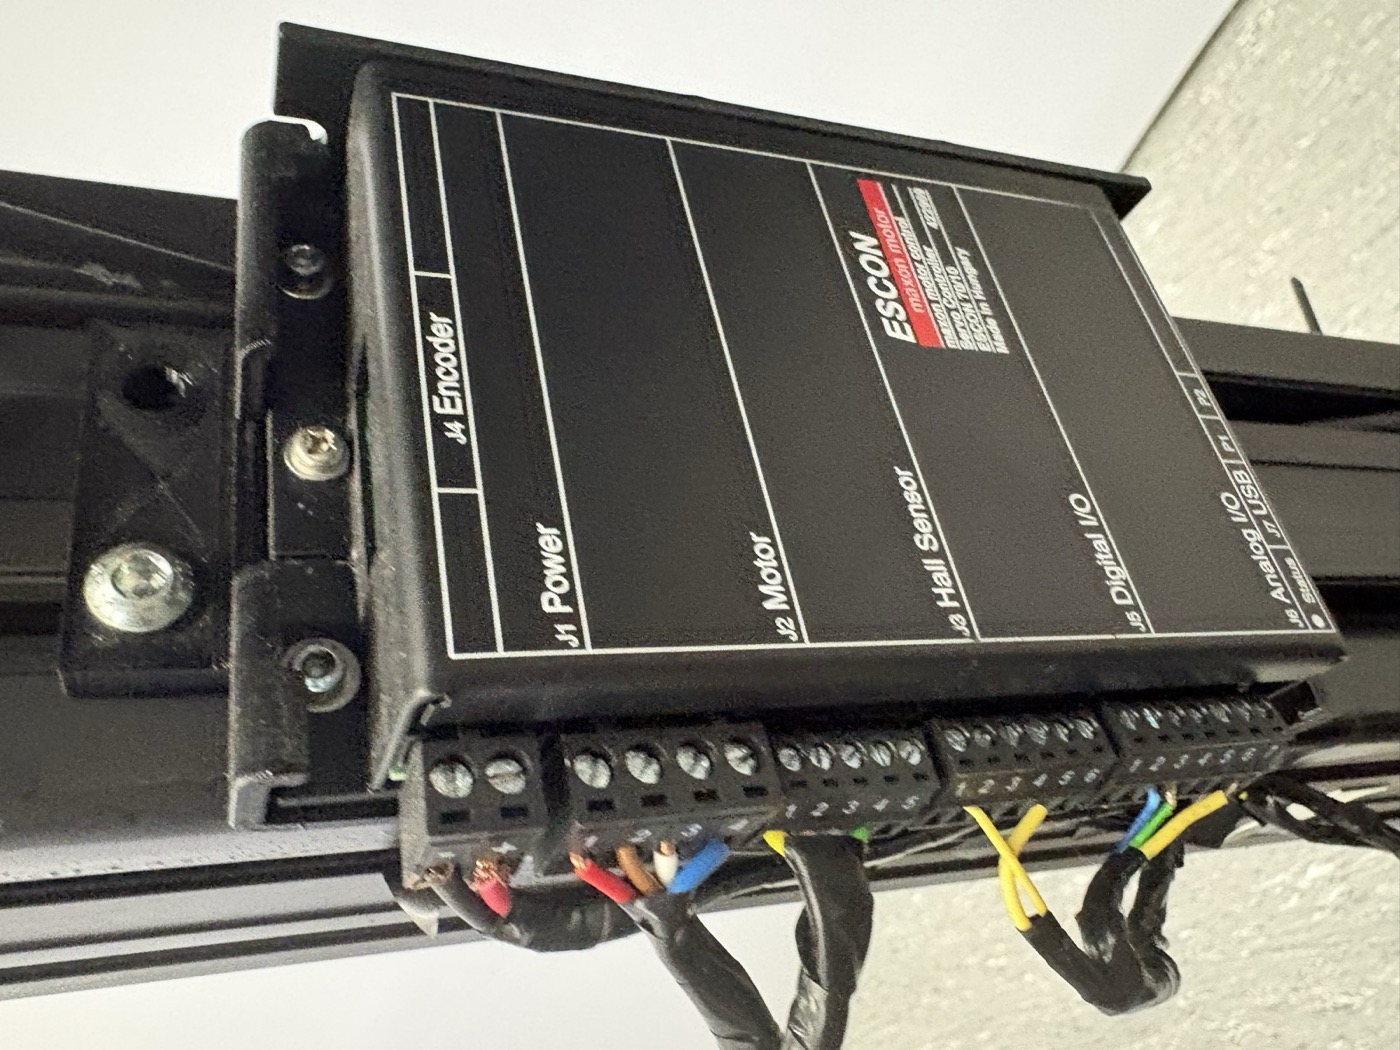
\includegraphics[width=\linewidth]{figures/2026-09-29_escon-7010-connectors.jpg}\\\small ESCON 70/10, terminal side
\end{minipage}\hfill
\begin{minipage}{0.32\linewidth}\centering
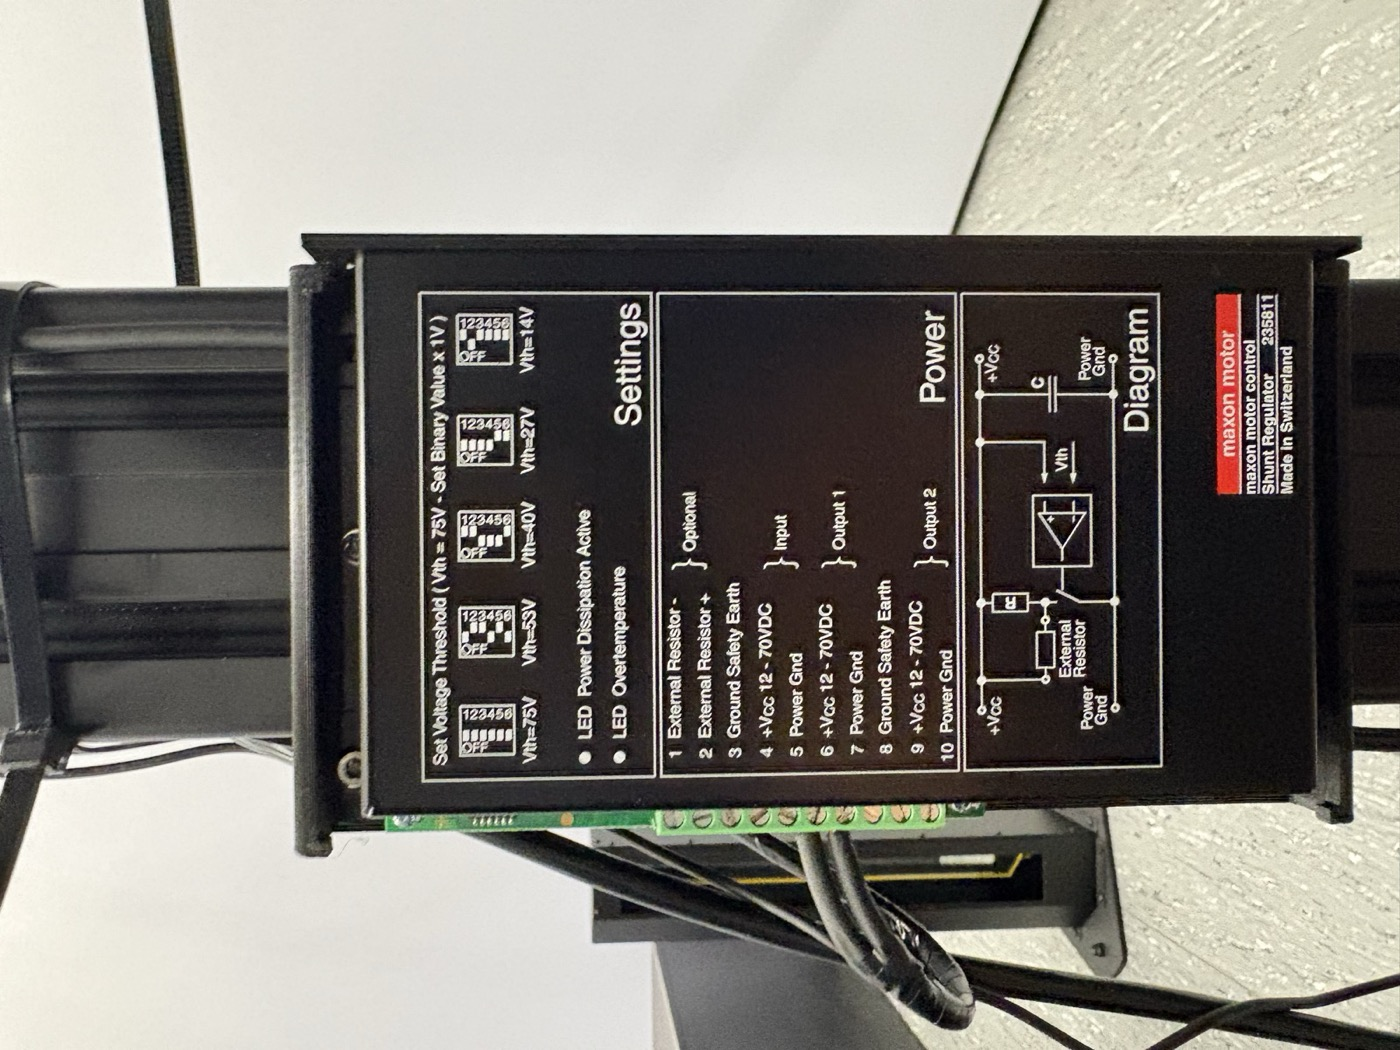
\includegraphics[width=\linewidth]{figures/2026-09-30_shunt-regulator.jpg}\\\small Brake chopper DSR 70/30
\end{minipage}\hfill
\begin{minipage}{0.32\linewidth}\centering
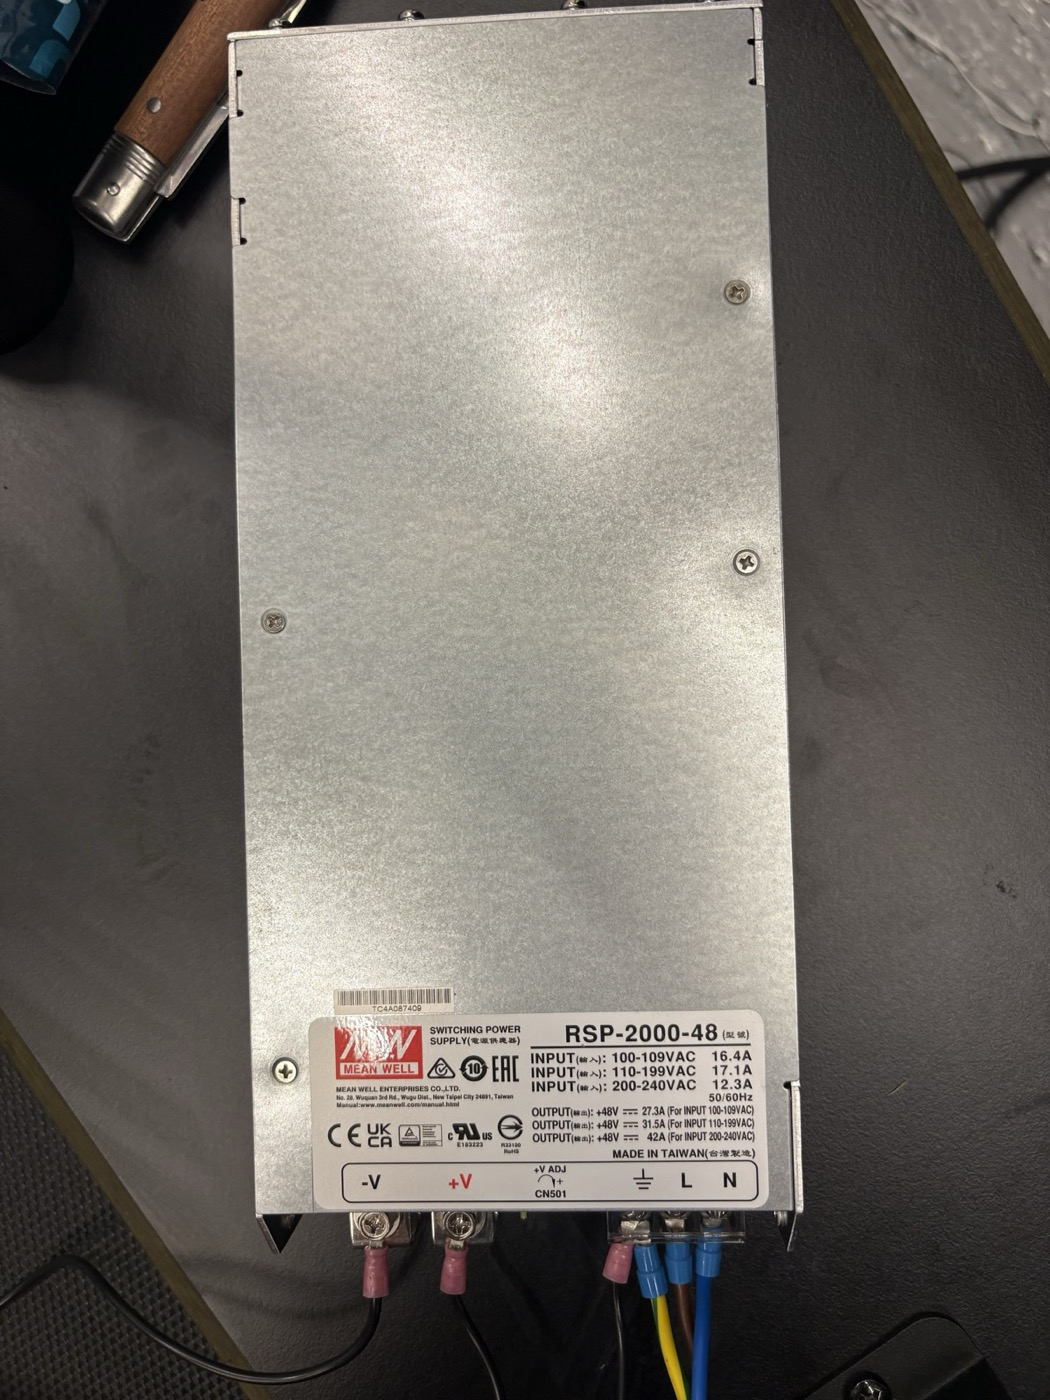
\includegraphics[width=\linewidth]{figures/2026-09-30_48V-psu-meanwell-rsp-2000-48.jpg}\\\small 48\,V supply RSP-2000-48
\end{minipage}
\caption{Per-tower power electronics (photos 29--30 Sep 2026).}
\end{figure}

\subsection{Material bought and to buy}
Prices are from the order or the shop page on the date given; check before ordering again.
Full lists: \file{docs/parts-list.xlsx} (one complete tower), \file{docs/parts-to-buy.xlsx}.

{\small
\begin{longtable}{>{\raggedright}p{4.2cm} >{\raggedright}p{4.0cm} >{\raggedright}p{2.2cm} >{\raggedright\arraybackslash}p{4.3cm}}
\toprule
Item & Part & Status & Why / note \\
\midrule\endhead
\bottomrule\endfoot
Motor driver, tower B & maxon ESCON 70/10, 422969 & ordered 7 Oct 2026 & old one: enable and USB dead. maxongroup.de, EUR 417.67 + EUR 14.90 shipping + VAT = EUR 514.76 \\
48\,V supply, tower B & Mean Well RSP-2000-48 & in use & old one faulty. \fillin{source / order} \\
Carrier PCB & \file{hardware/carrier/fab} & being made & HS Offenburg makerspace, bare copper, expected 16 Oct 2026 \\
Carrier parts & 2$\times$ female header 1$\times$24, 2$\times$ 1$\times$6; 4$\times$ Phoenix MSTB 2,5/5-GF-5,08 (1776537) + 4$\times$ plug MSTB 2,5/5-STF-5,08 (1778014); 4$\times$ 1\,k$\Omega$, 4$\times$ 1\,M$\Omega$, 4$\times$ BAT85 & to buy / makerspace & BOM \file{hardware/carrier/fab/bumpem-carrier-bom.csv} \\
Ferrules 0.25--0.5\,mm$^2$ & & to buy & 5 signal wires per module plug; never tin wire tips under a screw \\
Pin terminals, blue, 1.5--2.5\,mm$^2$ + crimper for insulated terminals & & to buy & 14\,AWG chopper $\rightarrow$ ESCON cable, tower B \\
Screws & M3$\times$6, M4$\times$12, M6$\times$16 ISO~7380, slot-10 T-nuts & to buy & printed parts (Sect.~\ref{sec:printed}); M6 length to confirm on the test print \\
E-stop & Hirose DF11-12DS housing + DF11 crimp terminals per 48\,V supply; button with one NO contact block per supply & to order & Sect.~\ref{sec:estop} \\
Load cell (spare) & DYMH-103, 100\,kg & only if needed & if the 200\,kg cell fails calibration \\
Brake chopper (spare) & maxon DSR 70/30, 235811 & not needed & tower B's chopper passed at 24\,V and 48\,V \\
\end{longtable}
}

Not bought, already in stock: motors, choppers (4), RSP-2000-48 (3 + B's), RS-15-24 (4), IAA100 (4),
load cells, Teensy 4.1, MCP4728, frame.

\subsection{Printed tower parts}\label{sec:printed}
To get the electronics off the floor and off tape, I designed printed holders that bolt into the profile
slots (\file{hardware/enclosures/}, CadQuery; overview \file{hardware/enclosures/out/parts-overview.pdf}).
All slot and bolt dimensions live in \file{tower.py}; device sizes come from the datasheets in
\file{docs/reference/}.

\begin{figure}[H]\centering
\begin{minipage}{0.24\linewidth}\centering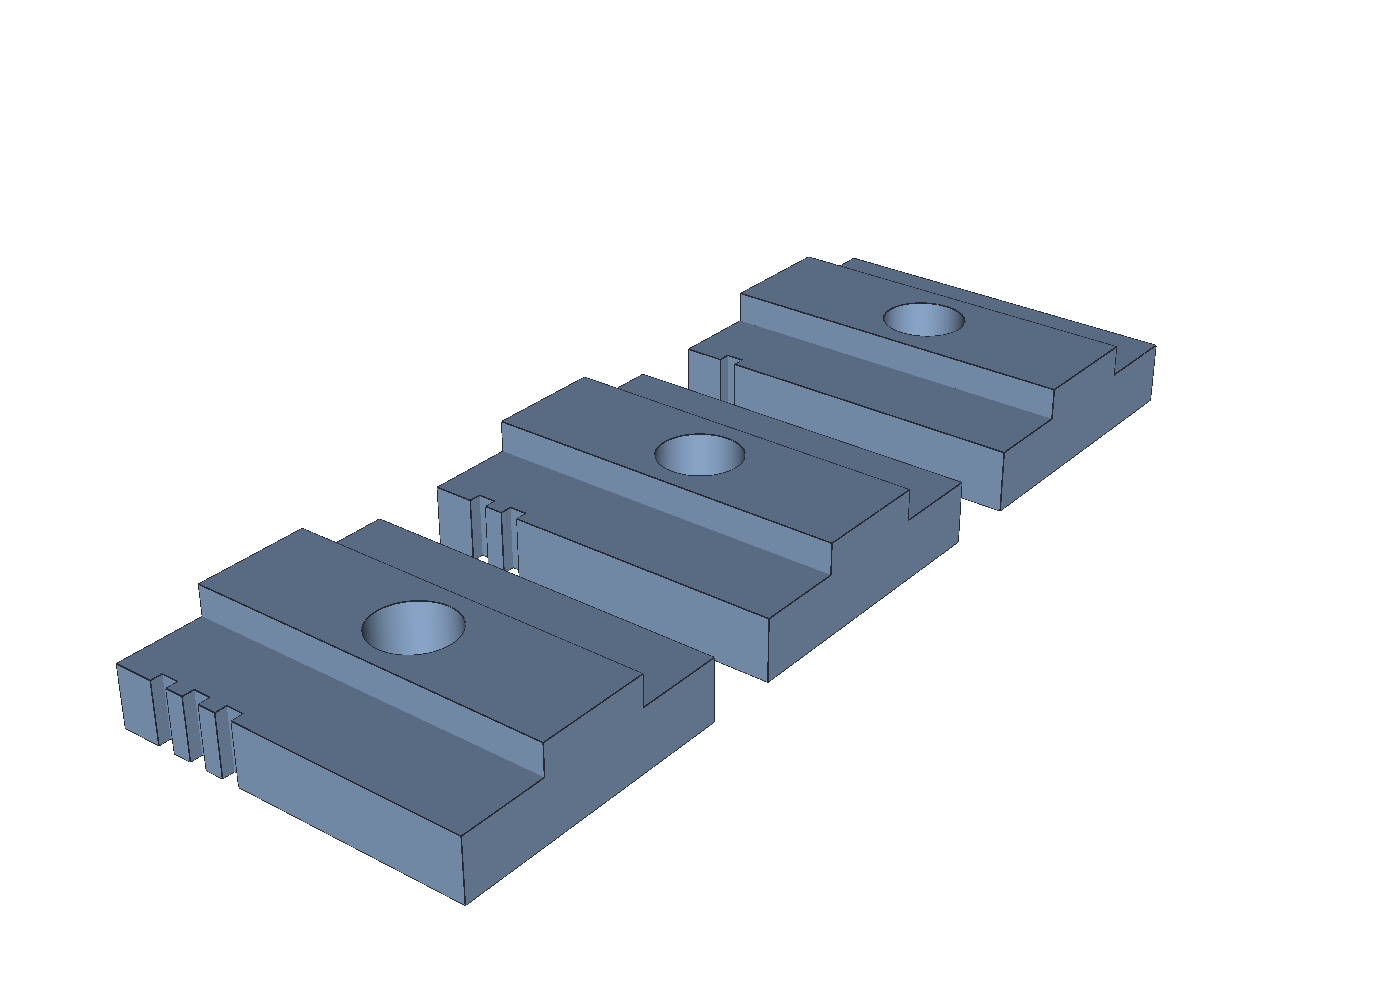
\includegraphics[width=\linewidth]{figures/render-testplates.png}\\\scriptsize slot test plates (0.1/0.2/0.3\,mm)\end{minipage}\hfill
\begin{minipage}{0.24\linewidth}\centering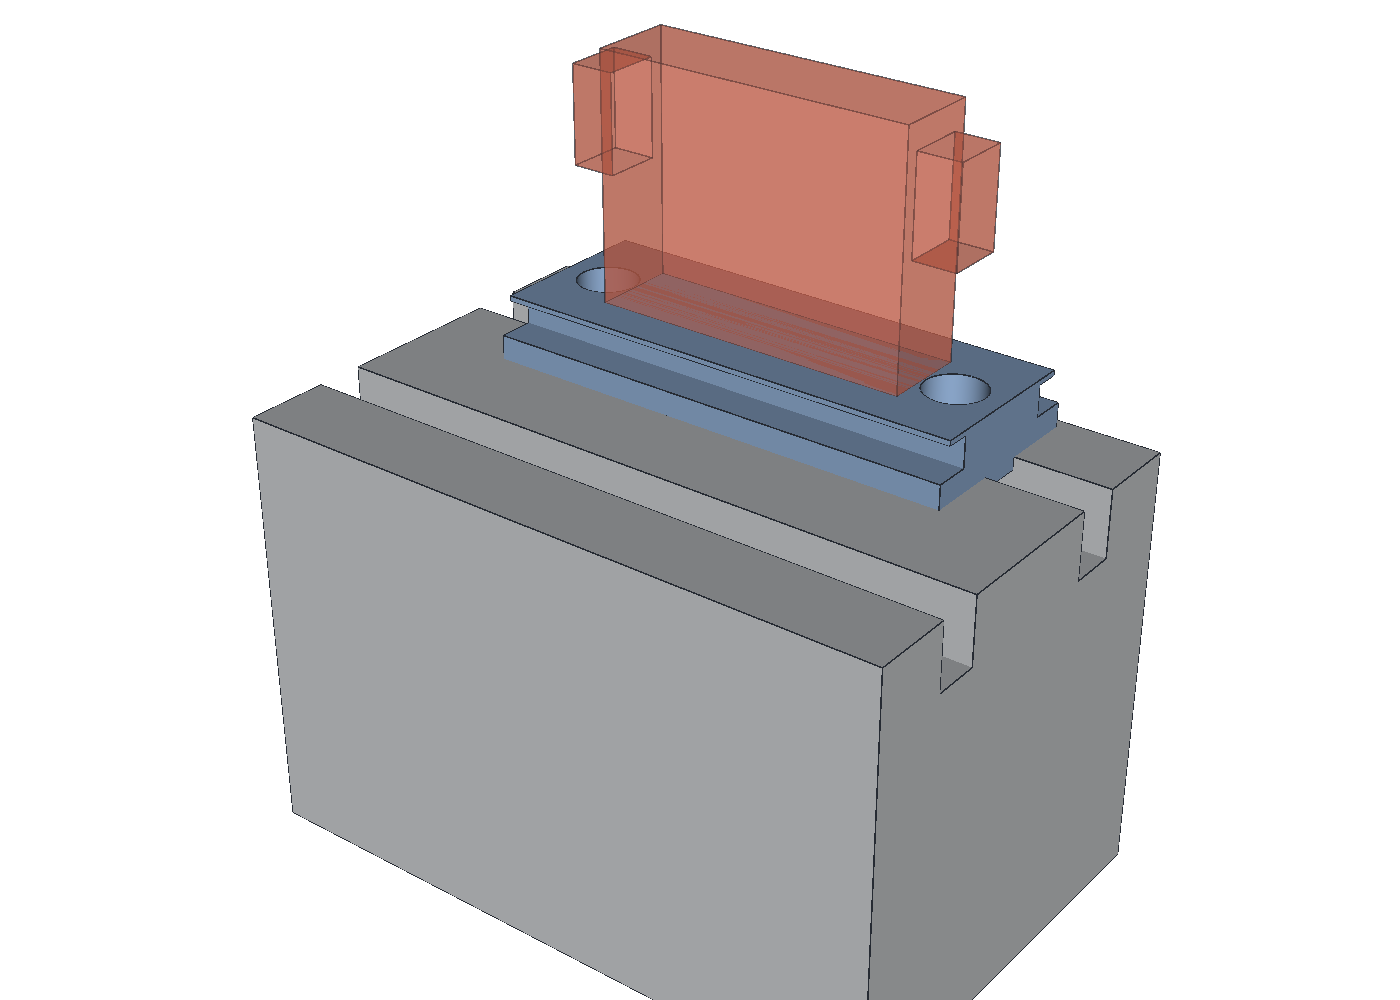
\includegraphics[width=\linewidth]{figures/render-iaa100.png}\\\scriptsize IAA100 on a printed DIN rail\end{minipage}\hfill
\begin{minipage}{0.24\linewidth}\centering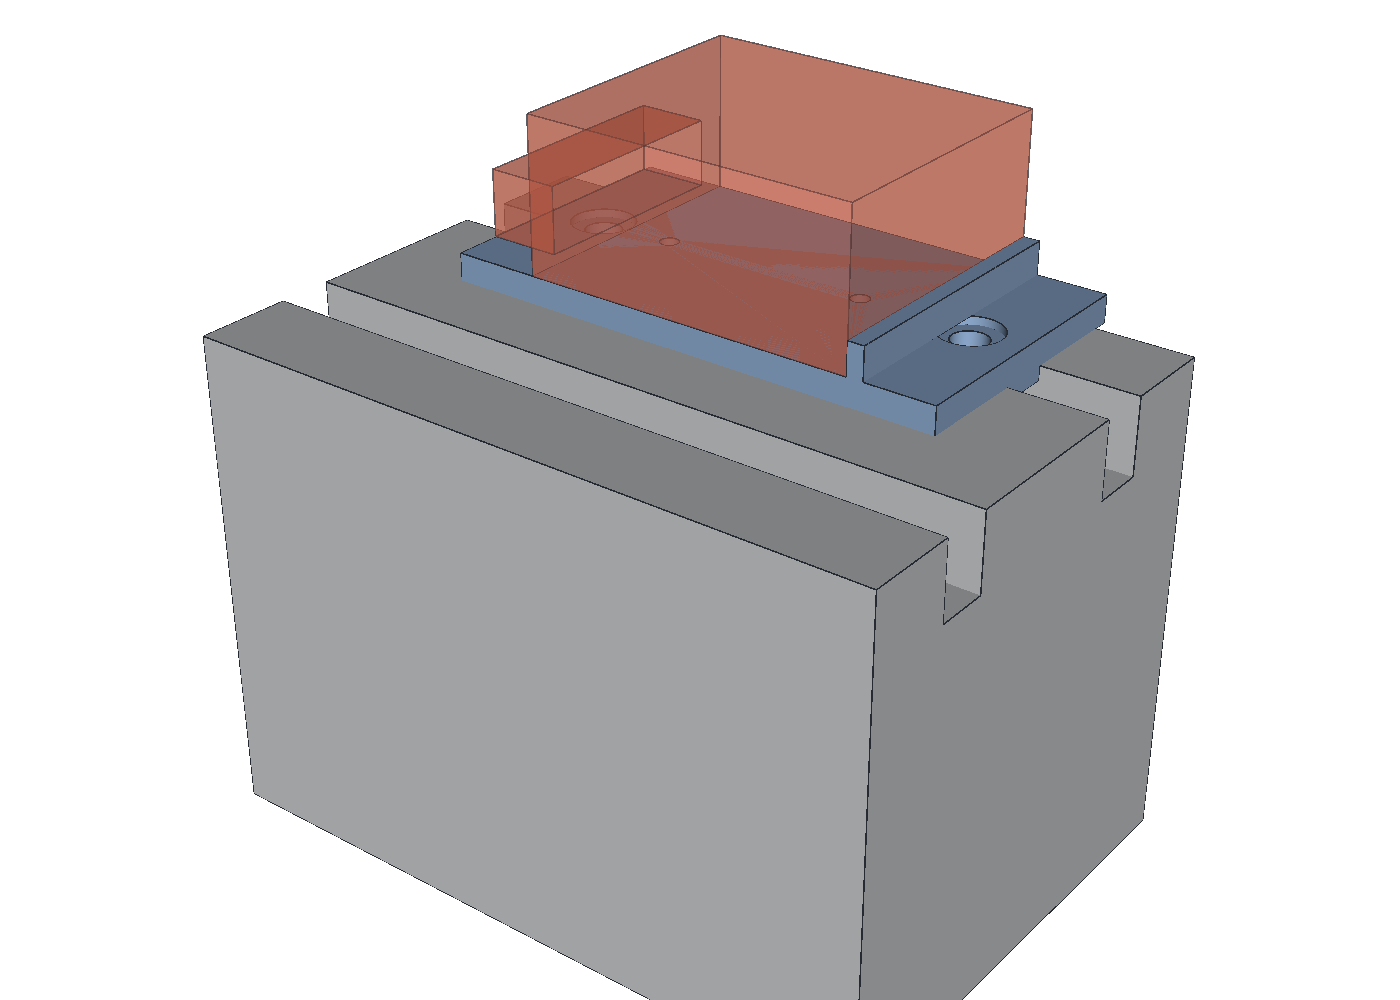
\includegraphics[width=\linewidth]{figures/render-rs15.png}\\\scriptsize RS-15-24 plate, 2$\times$M3$\times$6\end{minipage}\hfill
\begin{minipage}{0.24\linewidth}\centering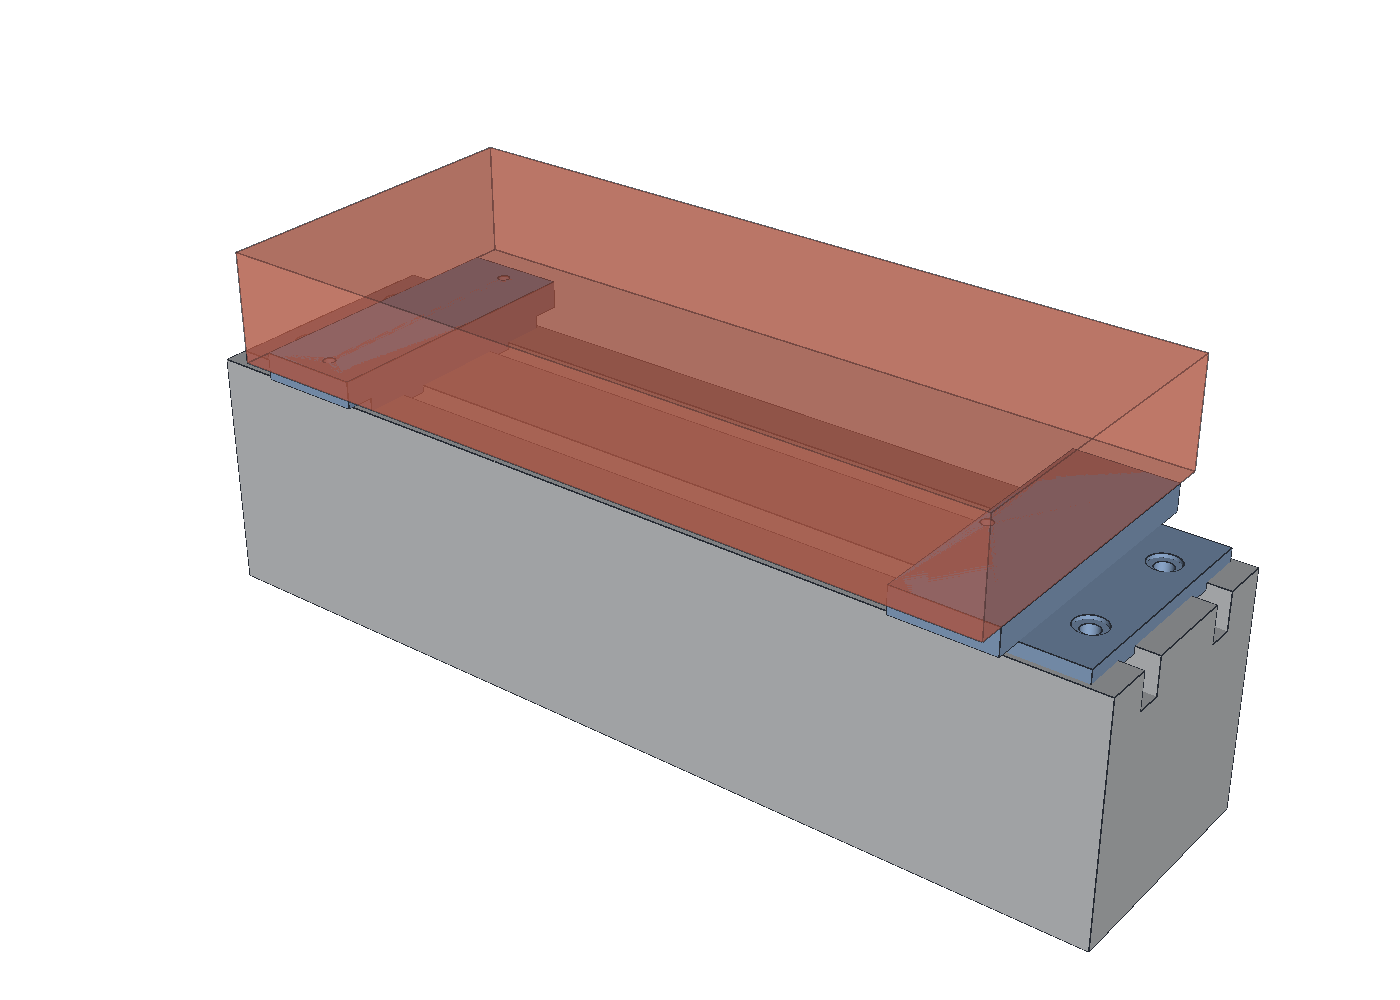
\includegraphics[width=\linewidth]{figures/render-rsp2000.png}\\\scriptsize RSP-2000 brackets, M4$\times$12, 10\,mm air gap\end{minipage}
\caption{Printed parts. Print PETG or ASA (48\,V brackets: ASA, or PETG $\geq$ 40\,\% infill).}
\end{figure}

To change a part: edit \file{tower.py} or \file{parts.py}, then run \cmd{python make\_stl.py} and
\cmd{python overview.py} in that folder (needs \cmd{pip install cadquery matplotlib vtk}). After the test
print, set \cmd{KEY\_CLEAR} in \file{tower.py} to the plate that slid in without play (currently 0.2\,mm).

\section{Cabling maps}\label{sec:cabling}

Text source of everything here: \file{docs/knowledge/wiring.md} and \file{escon/README.md}. Pin numbers
are from the maxon, Futek and Mean Well datasheets in \file{docs/reference/} and \file{escon/}.

\warn{The 230\,V side of both supplies (L, N, earth) is electrician work only. Before touching anything on
the 48\,V side: mains off, then measure the chopper pins 4--5 below 1\,V (it holds 8800\,\textmu F).}

\subsection{Power chain per tower}\label{sec:power}

\begin{figure}[H]\centering
\resizebox{\linewidth}{!}{%
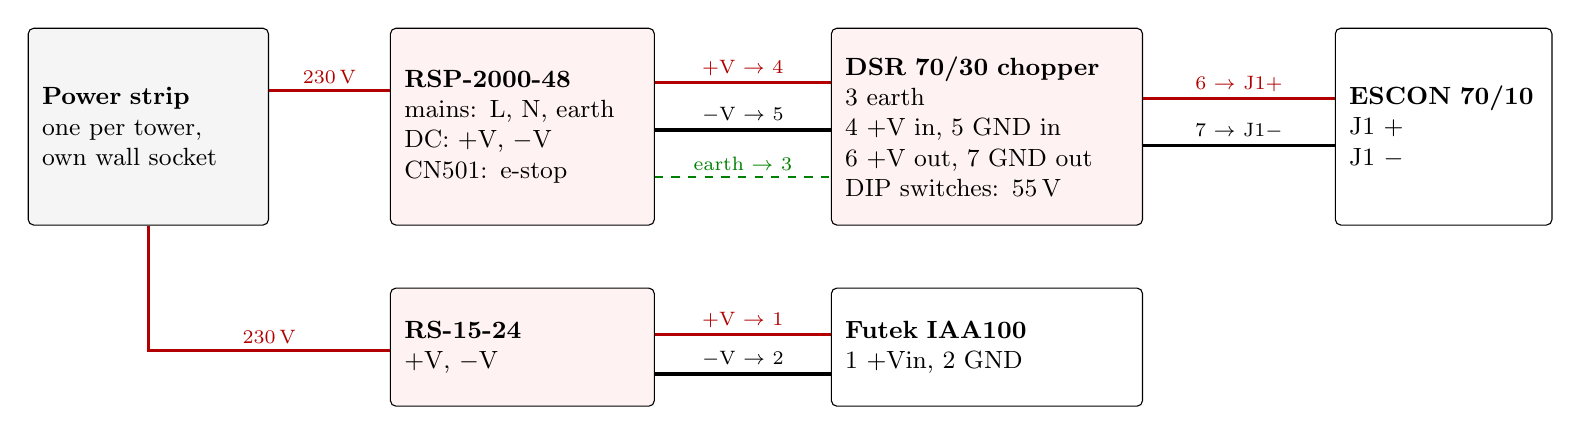
\begin{tikzpicture}[
  box/.style={draw, rounded corners=2pt, align=left, font=\small, inner sep=5pt, anchor=north west},
  pwr/.style={very thick, red!70!black},
  gnd/.style={very thick, black},
  pe/.style={thick, green!50!black, dashed},
  lab/.style={font=\scriptsize, above, inner sep=2pt}]
  \newcommand{\wire}[5]{\draw[#1] ($(#2.north east)+(0,#4)$) -- node[lab]{#5} ($(#3.north west)+(0,#4)$);}
  \node[box, fill=black!4, text width=2.7cm, minimum height=2.5cm] (strip) at (0,0) {\textbf{Power strip}\\one per tower,\\own wall socket};
  \node[box, fill=red!5, text width=3.0cm, minimum height=2.5cm] (psu) at (4.6,0) {\textbf{RSP-2000-48}\\mains: L, N, earth\\DC: +V, $-$V\\CN501: e-stop};
  \node[box, fill=red!5, text width=3.6cm, minimum height=2.5cm] (chop) at (10.2,0) {\textbf{DSR 70/30 chopper}\\3 earth\\4 +V in, 5 GND in\\6 +V out, 7 GND out\\DIP switches: 55\,V};
  \node[box, text width=2.4cm, minimum height=2.5cm] (escon) at (16.6,0) {\textbf{ESCON 70/10}\\J1 +\\J1 $-$};
  \wire{pwr}{strip}{psu}{-0.8}{230\,V}
  \wire{pwr}{psu}{chop}{-0.7}{+V $\rightarrow$ 4}
  \wire{gnd}{psu}{chop}{-1.3}{$-$V $\rightarrow$ 5}
  \wire{pe}{psu}{chop}{-1.9}{earth $\rightarrow$ 3}
  \wire{pwr}{chop}{escon}{-0.9}{6 $\rightarrow$ J1+}
  \wire{gnd}{chop}{escon}{-1.5}{7 $\rightarrow$ J1$-$}
  \node[box, fill=red!5, text width=3.0cm, minimum height=1.5cm] (rs) at (4.6,-3.3) {\textbf{RS-15-24}\\+V, $-$V};
  \node[box, text width=3.6cm, minimum height=1.5cm] (amp) at (10.2,-3.3) {\textbf{Futek IAA100}\\1 +Vin, 2 GND};
  \draw[pwr] ($(strip.south)$) |- node[lab, pos=0.75]{230\,V} ($(rs.north west)+(0,-0.8)$);
  \wire{pwr}{rs}{amp}{-0.6}{+V $\rightarrow$ 1}
  \wire{gnd}{rs}{amp}{-1.1}{$-$V $\rightarrow$ 2}
\end{tikzpicture}}
\caption{Power wiring of one tower (Stanford guide pp.\,14--16, chopper and supply datasheets). Mains side: electrician only.}
\label{fig:power}
\end{figure}

\begin{itemize}
\item \textbf{One power strip per tower, each on its own wall socket.} Never plug a strip into a strip: an
RSP-2000 draws up to 50\,A inrush and about 10\,A at full load (DGUV rules).
\item The RSP-2000 has no switch: it is on whenever its mains cable is live.
\item Chopper $\rightarrow$ ESCON cable: Stanford uses 14\,AWG ($\approx$ 2\,mm$^2$). The chopper terminals take
0.14--1.5\,mm$^2$, ESCON J1 takes 0.2--2.5\,mm$^2$. Crimp blue insulated pin terminals (1.5--2.5\,mm$^2$,
pin $\approx$ 1.9\,mm; try one in the chopper first) with a crimper for insulated terminals, or use 1.5\,mm$^2$
wire with 1.5\,mm$^2$ ferrules. A ferrule crimper does not crimp pin terminals.
\item Open on tower B (electrician): earth wire supply $\rightarrow$ chopper terminal 3; cover for the
RS-15-24's open 230\,V terminals.
\end{itemize}

\subsection{ESCON 70/10 connectors}

\begin{table}[H]\centering\small
\begin{tabularx}{\linewidth}{llX}
\toprule
Connector & Pin & Use in Bump'em \\
\midrule
J1 Power & +, $-$ & 48\,V from chopper pins 6 / 7 \\
J2 Motor & 1, 2, 3 & windings 1, 2, 3: red, brown, white \\
         & 4 & cable shield: \textbf{empty} \\
J3 Hall  & 1, 2, 3 & Hall 1, 2, 3: yellow, pink, grey \\
         & 4, 5 & +5\,V Hall supply: green; GND: blue \\
J5 Digital I/O & 2 & DigIN2 = \textbf{enable} $\leftarrow$ Teensy 27/28/29/30 (yellow) \\
               & 5 & GND $\rightarrow$ ground distributor \\
               & 6 & +5\,V out: \textbf{never to a Teensy pin} \\
J6 Analog I/O  & 3, 4 & AnIN2+ / AnIN2$-$ = \textbf{setpoint} $\leftarrow$ DAC VA--VD (blue) / DAC GND (green) \\
               & 5, 6 & analog outputs, $-4$\ldots$+4$\,V: \textbf{never to a Teensy pin} \\
               & 7 & GND $\rightarrow$ ground distributor \\
J7 USB & & ESCON Studio (Windows) for configuration only \\
\bottomrule
\end{tabularx}
\caption{ESCON pins (hardware reference Tables 3-12, 3-17, 3-19). J2/J3 colours as found on module C;
check every module against this table before the first drive.}
\end{table}

\paragraph{Motor connector.} The EC 90 flat 500267 has one 8-pin Molex connector: 1 Hall 1, 2 Hall 2,
3 V\textsubscript{Hall}, 4 winding 3, 5 Hall 3, 6 Hall GND, 7 winding 1, 8 winding 2
(\file{docs/reference/maxon-500267-catalog-page.pdf}). Hall GND (blue) belongs on J3 pin 5, not on the J2
shield pin; two modules had it wrong (Sect.~\ref{sec:lessons}).

\begin{figure}[H]\centering
\begin{minipage}{0.48\linewidth}\centering
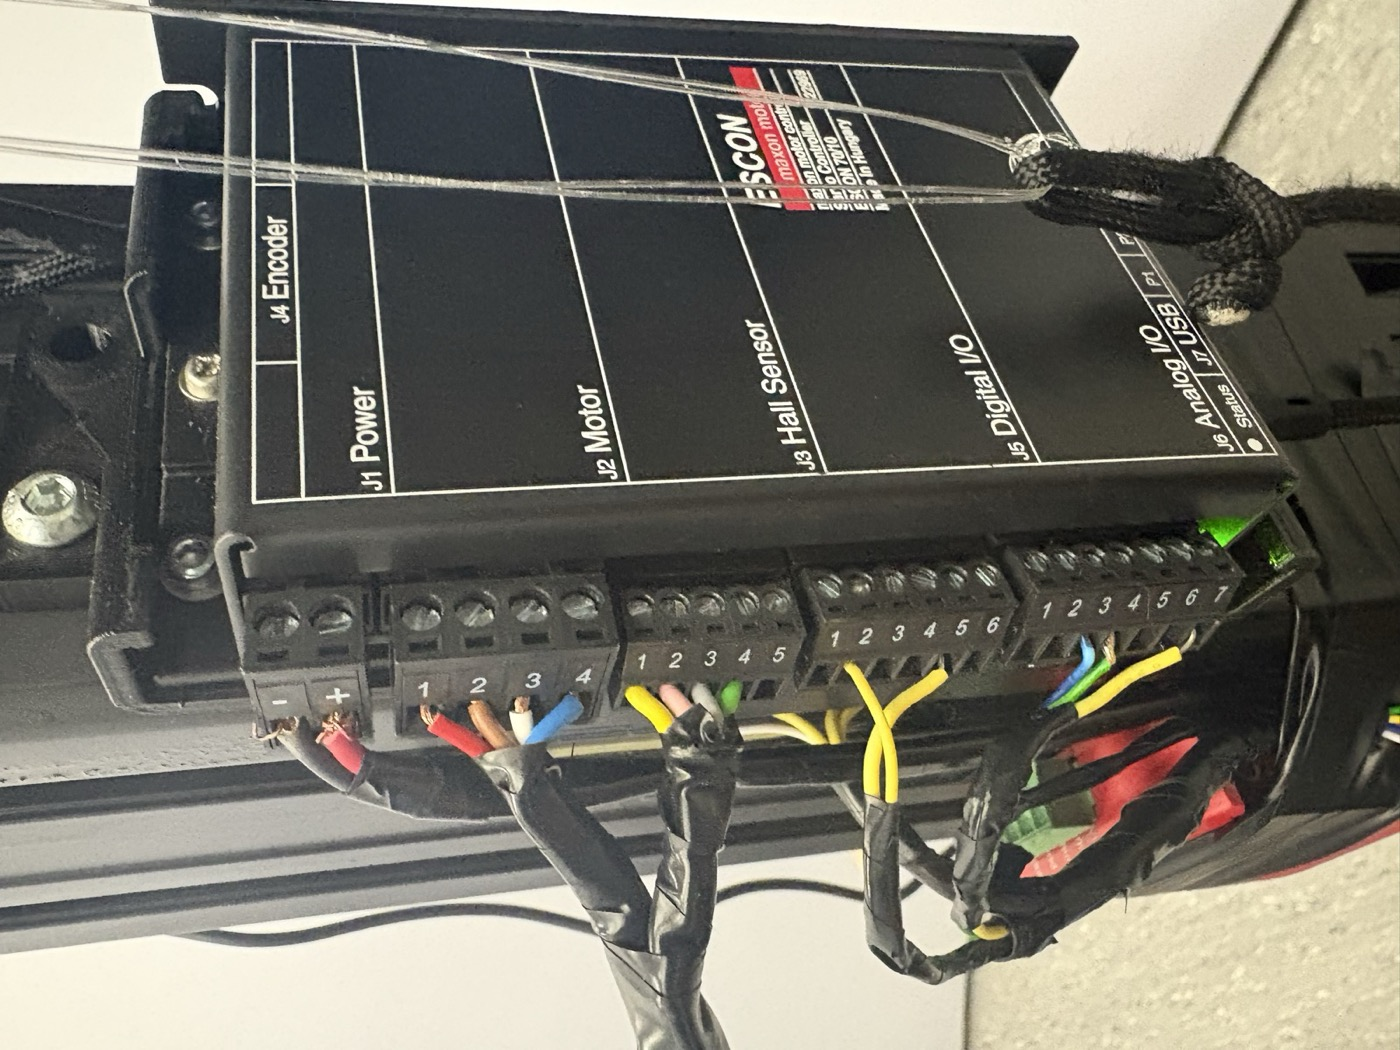
\includegraphics[width=\linewidth]{figures/2026-10-01_escon-moduleC-all-connectors.jpg}\\\small Module C, all plugs readable (before the Hall GND fix)
\end{minipage}\hfill
\begin{minipage}{0.48\linewidth}\centering
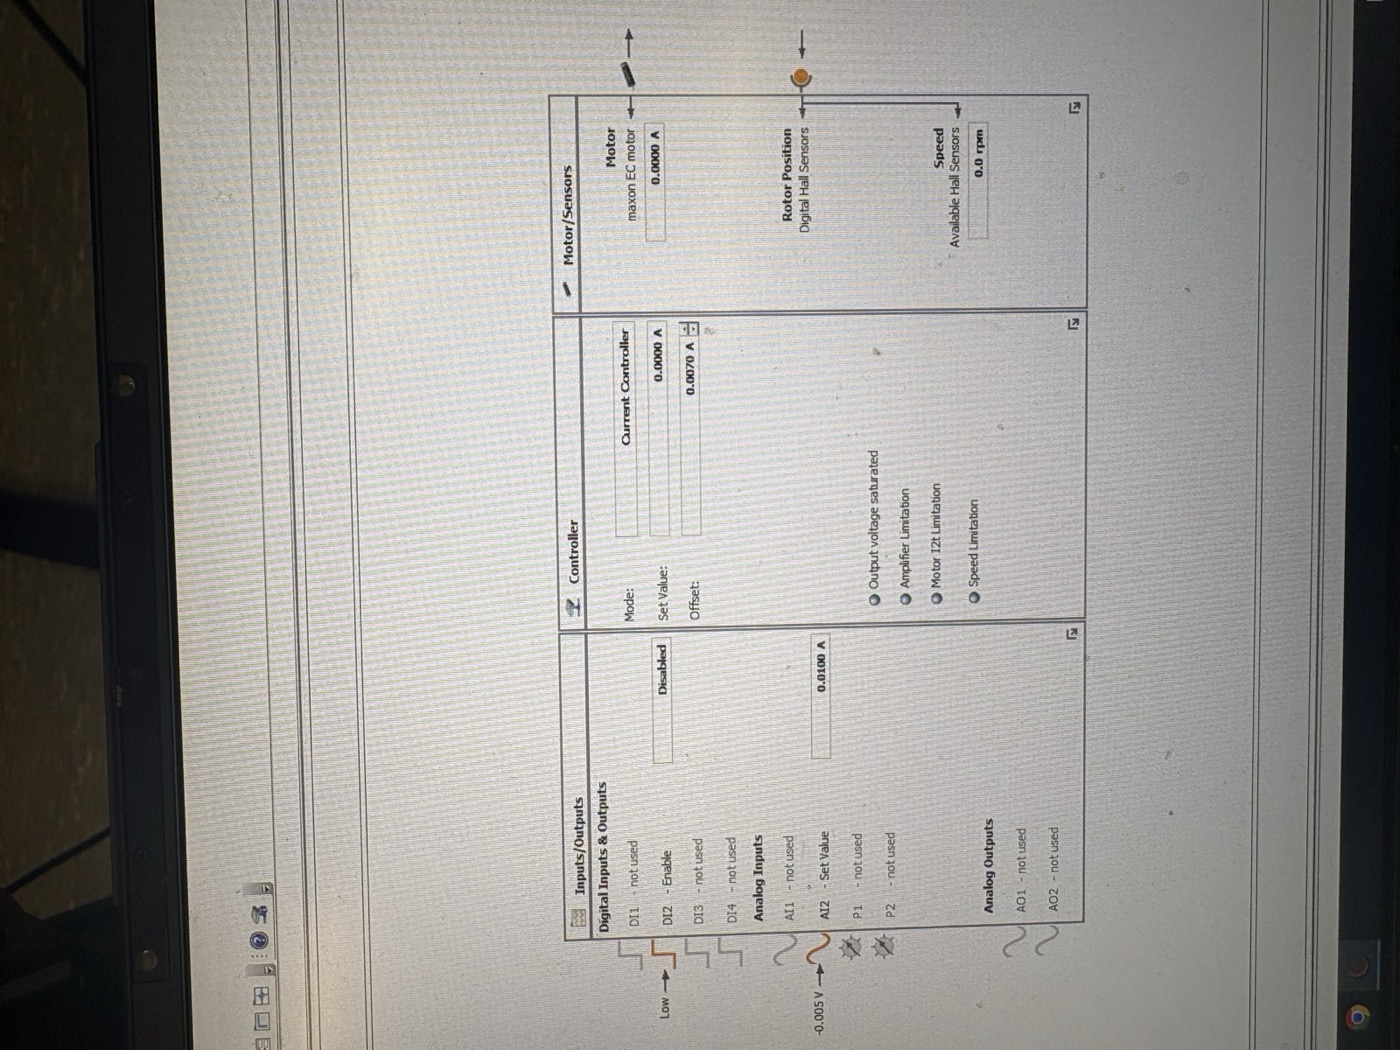
\includegraphics[width=\linewidth]{figures/2026-10-01_escon-studio-controller-monitor-moduleC.jpg}\\\small ESCON Studio controller monitor, module C
\end{minipage}
\end{figure}

\paragraph{Futek IAA100.} Power side (5-way): 1 +Vin 12.5--26\,V, 2 GND (power), 3 shunt cal (empty),
4 GND (output), 5 Vout. Sensor side (4-way): 1 +excitation, 2 +signal, 3 $-$signal,
4 $-$excitation or shield.
Vout (brown) goes to the Teensy force pin, output GND to the ground distributor.

\subsection{Control board $\leftrightarrow$ modules}

\begin{table}[H]\centering\small
\begin{tabular}{lllcccc}
\toprule
Wire & Colour & ESCON / amplifier end & A & B & C & D \\
\midrule
EN  & \textcolor{wyellow}{\rule{1.2em}{0.6em}} yellow & ESCON J5.2 (DigIN2) & T27 & T28 & T29 & T30 \\
SP+ & \textcolor{wblue}{\rule{1.2em}{0.6em}} blue   & ESCON J6.3 (AnIN2+) & VA & VB & VC & VD \\
SP$-$ & \textcolor{wgreen}{\rule{1.2em}{0.6em}} green & ESCON J6.4 (AnIN2$-$) & GND & GND & GND & GND \\
GND & \textcolor{wwhite}{\rule{1.2em}{0.6em}} white  & ground distributor & GND & GND & GND & GND \\
F   & \textcolor{wbrown}{\rule{1.2em}{0.6em}} brown  & IAA100 Vout & T14 & T15 & T16 & T17 \\
\bottomrule
\end{tabular}
\caption{Five wires per module (T = Teensy pin, V = DAC output). Pink and black in the same cable are
spares, taped. Shared once: Teensy 3V $\rightarrow$ DAC VCC, G $\rightarrow$ DAC GND, 19 $\rightarrow$ SCL,
18 $\rightarrow$ SDA. The Teensy 5V pin stays unconnected.}
\end{table}

\begin{figure}[H]\centering
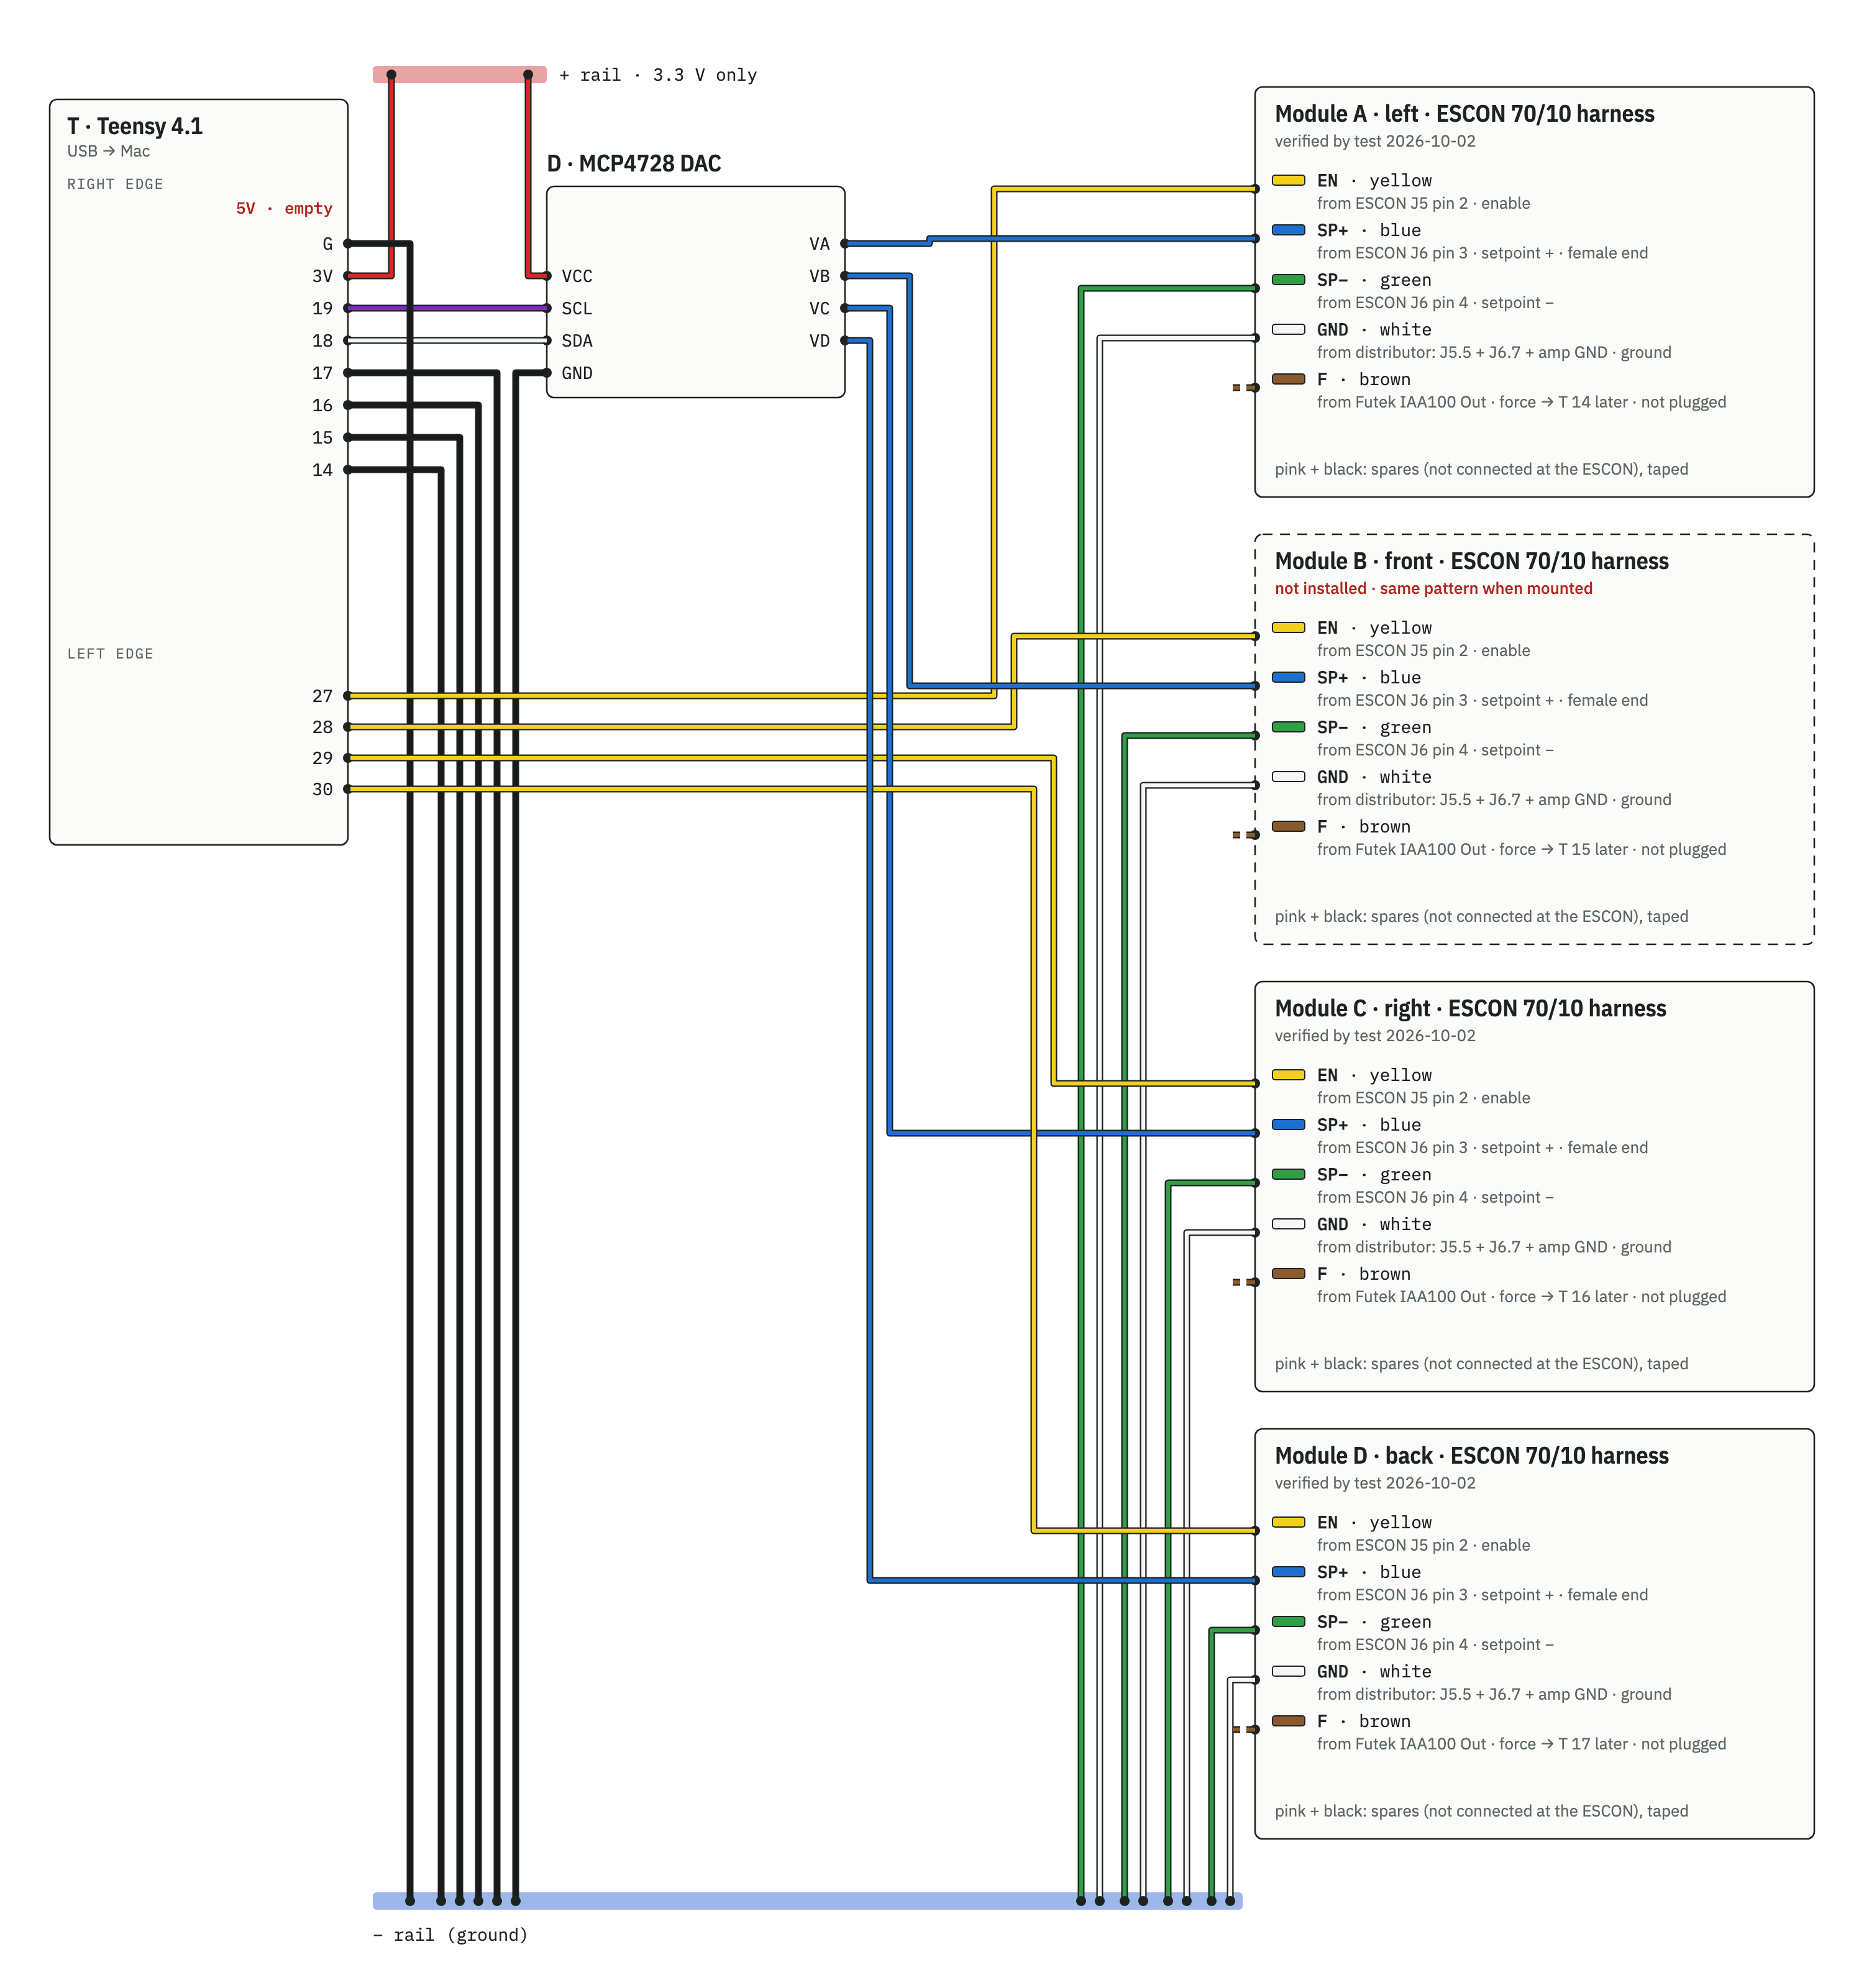
\includegraphics[width=0.78\linewidth]{figures/cabling-4-modules.png}
\caption{Breadboard cabling as of 2 Oct 2026 (\file{docs/diagrams/cabling-4-modules.png}). Since then B is
wired the same way and the brown force wires are plugged in. Valid until the carrier board replaces the
breadboard.}
\end{figure}

\subsection{Carrier PCB}\label{sec:carrier}
The breadboard was the cause of several faults (loose contacts, a wire on the wrong rail). The carrier
board (\file{hardware/carrier/}) holds the Teensy and DAC in sockets and gives each module one pluggable
5-way Phoenix MSTB connector: the module's wires are screwed into its plug once, the plug locks with two
flange screws.

\begin{figure}[H]\centering
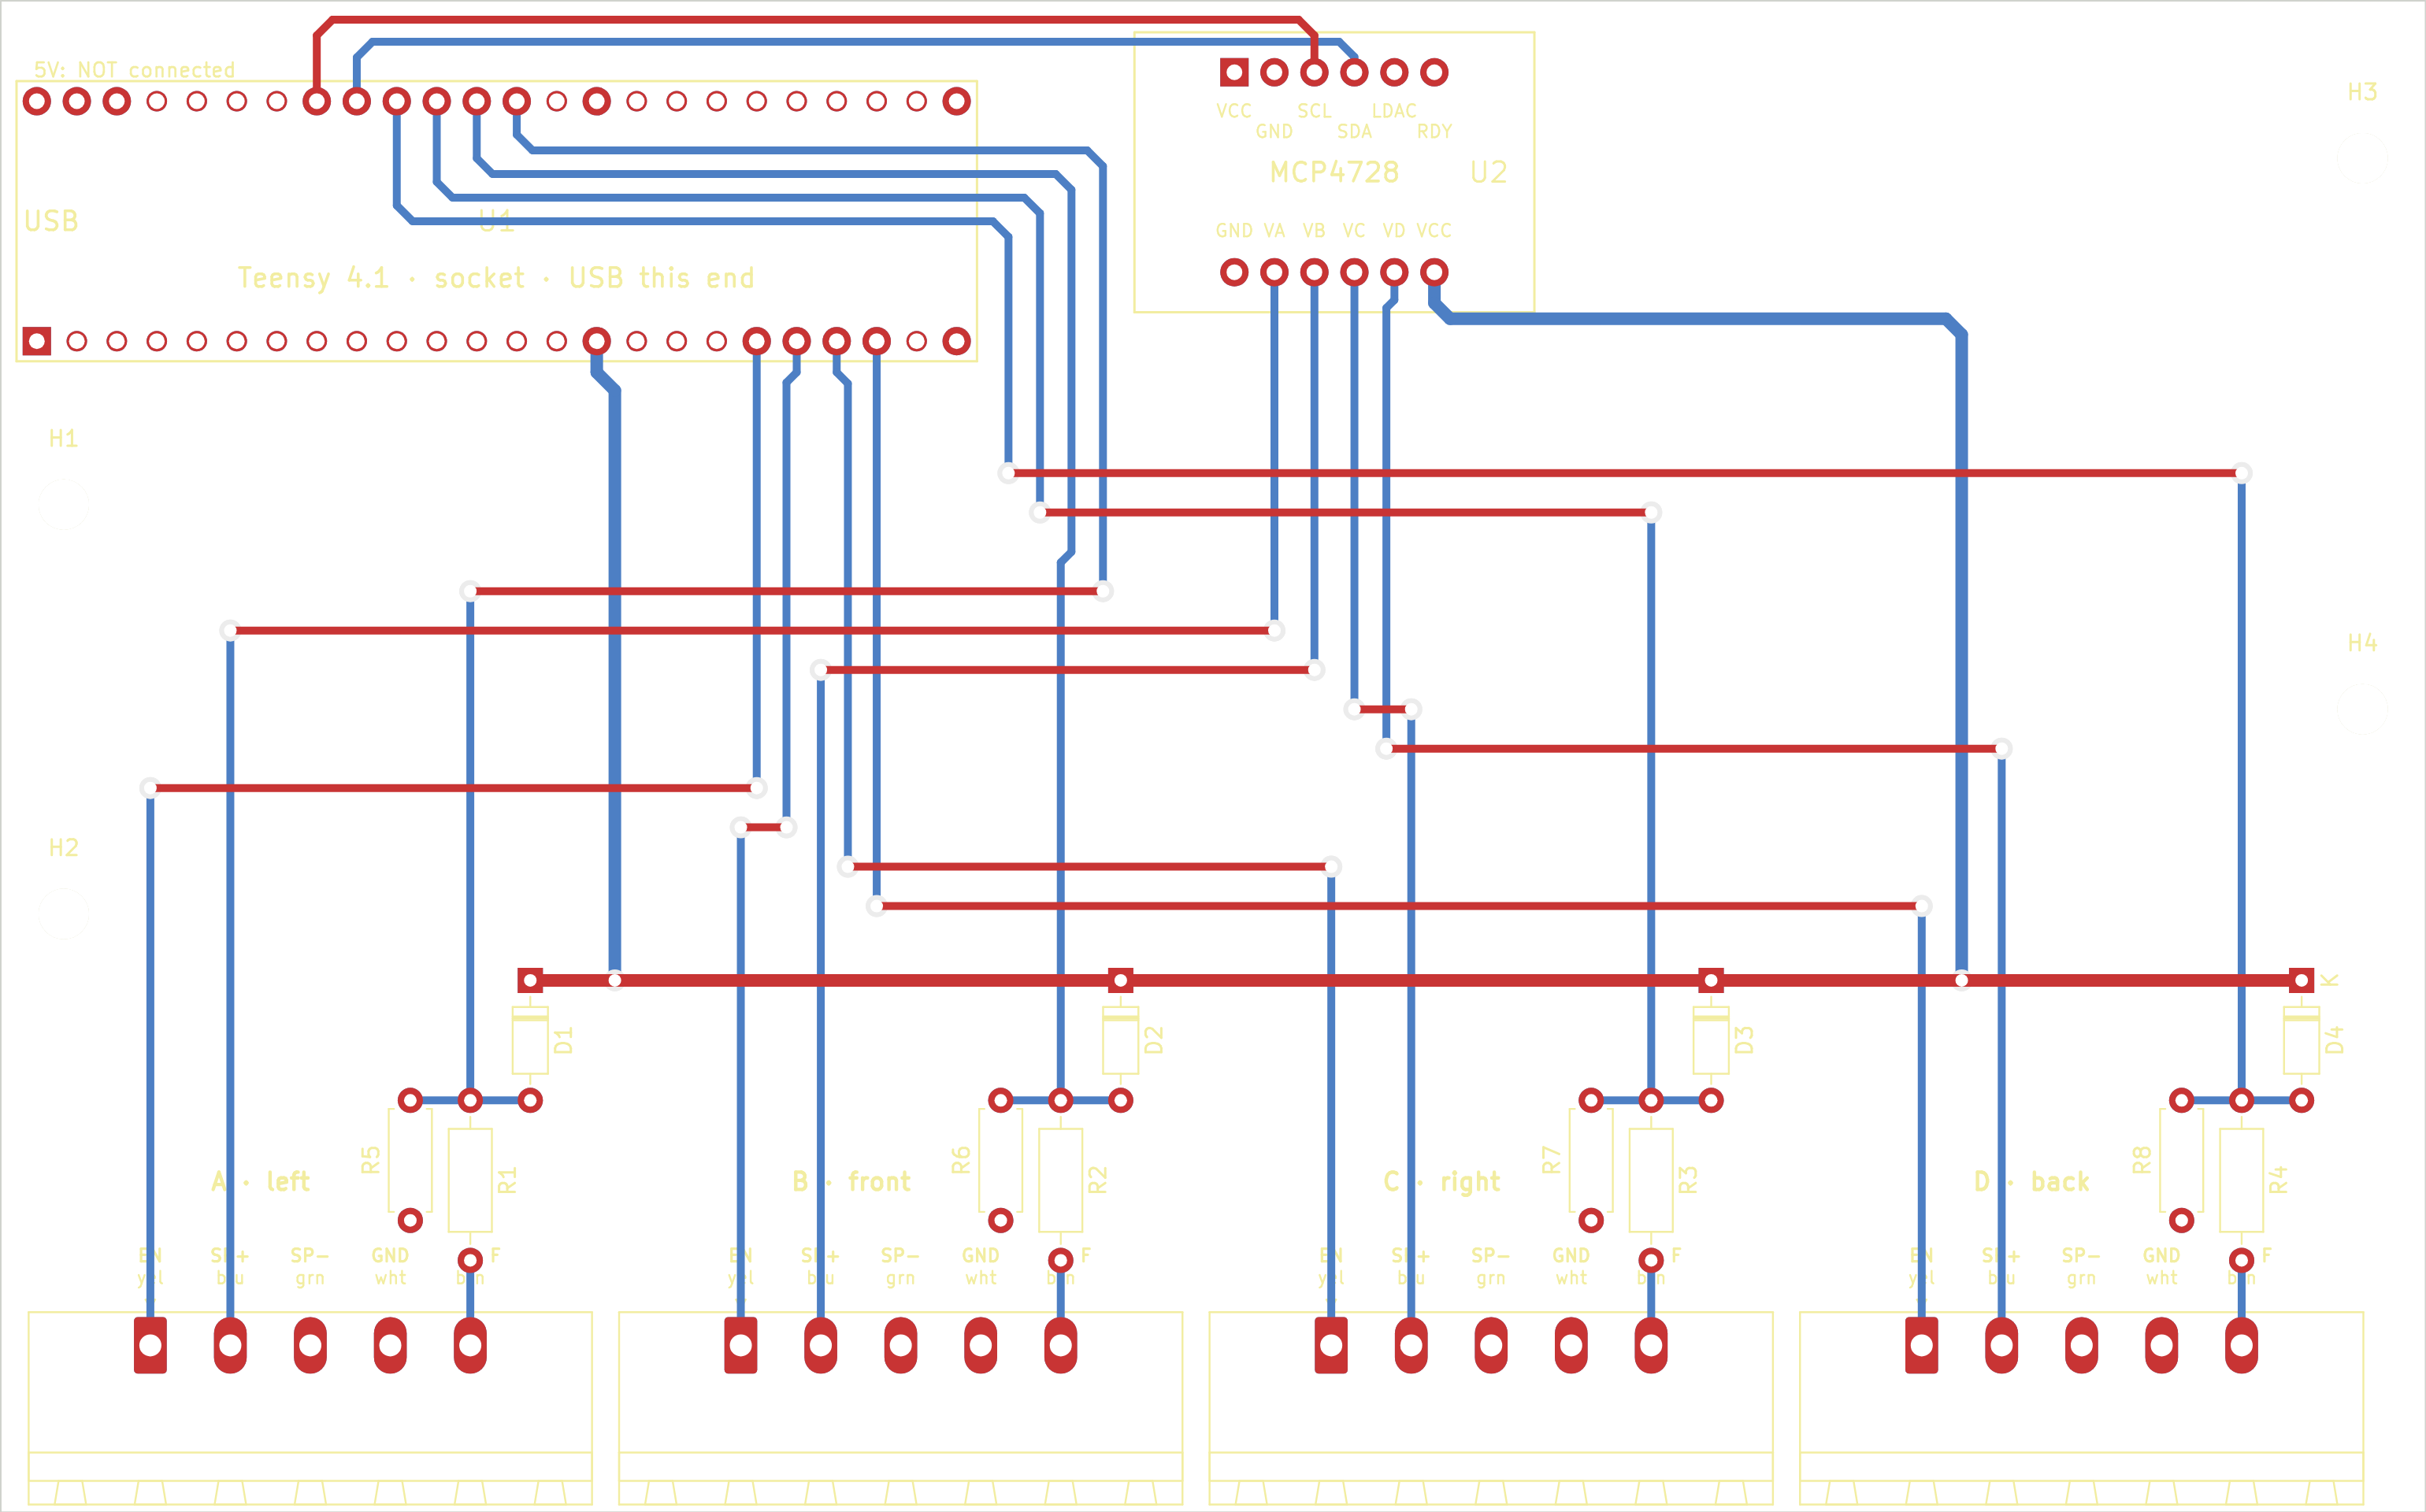
\includegraphics[width=0.85\linewidth]{figures/board-preview.png}
\caption{Carrier board v1, 154$\times$96\,mm, 2 layers, through-hole only. Red: top copper, blue: bottom.
Module plugs J1--J4 (A, B, C, D) at the bottom edge, pins left to right: 1 EN, 2 SP+, 3 SP$-$, 4 GND, 5 F.}
\end{figure}

\paragraph{Force input protection.} Per force input: connector F $\rightarrow$ 1\,k$\Omega$ $\rightarrow$
Teensy pin, 1\,M$\Omega$ to GND, BAT85 diode to 3.3\,V. The Teensy still sees 99.9\,\% of the amplifier
voltage, an unplugged input reads 0\,N, and an amplifier set above 3.3\,V cannot damage the Teensy pin. If an
amplifier can only be set to 0--10\,V, change the pair to a divider (e.g.\ 22\,k$\Omega$ / 10\,k$\Omega$) and
recalibrate.

\paragraph{Changing the board.} Never edit the KiCad files by hand; they are generated. Connections and
values: \file{netlist.py}; placement and routing: \file{gen_carrier.py}; schematic: \file{gen_schematic.py}.
Run \cmd{./build.sh} (KiCad 8): it must report 0 ERC, 0 DRC and 0 parity violations, and it rewrites the
gerber zip and PDFs in \file{fab/}.

\begin{figure}[H]\centering
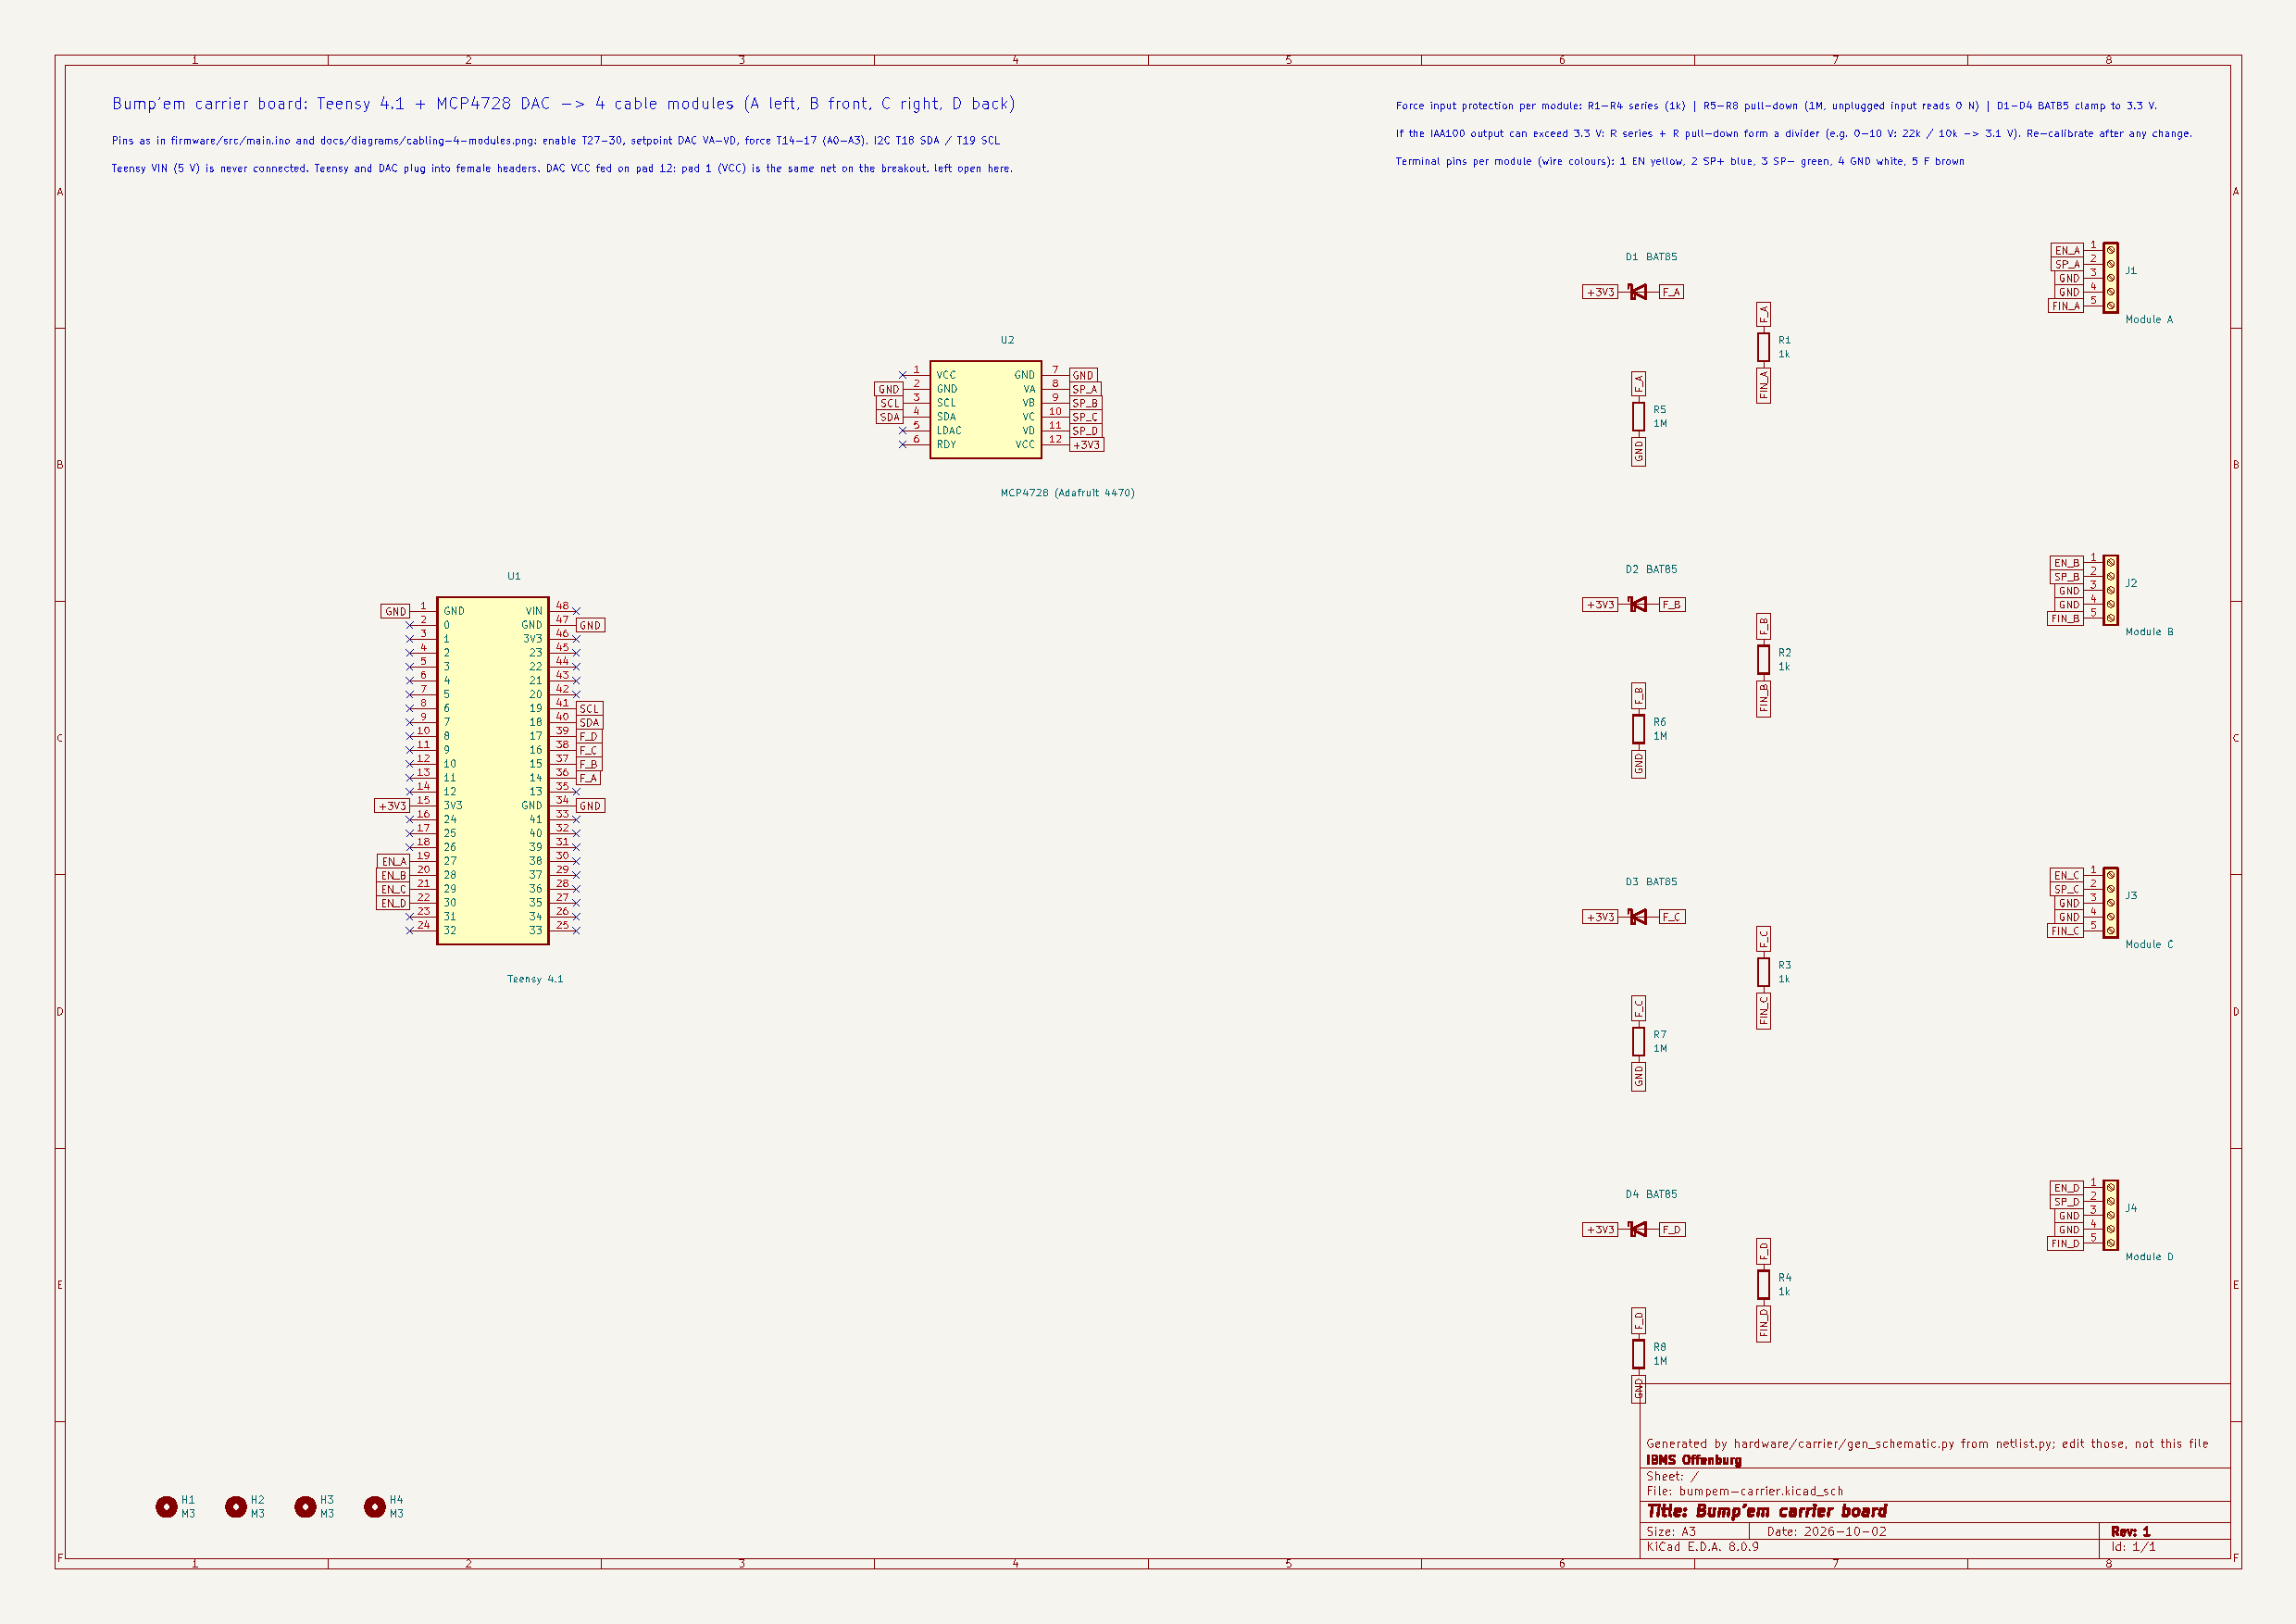
\includegraphics[width=\linewidth]{figures/carrier-schematic.pdf}
\caption{Carrier board schematic (\file{hardware/carrier/fab/bumpem-carrier-schematic.pdf}).}
\end{figure}

\subsection{E-stop (to be wired)}\label{sec:estop}
Stanford's e-stop switches off the 48\,V output of each RSP-2000 through its control connector CN501
(Hirose DF11-12DP):
\begin{itemize}
\item One button with one \textbf{normally open} contact block per 48\,V supply (four towers = four NO blocks
on one button, each pair of wires kept separate).
\item Per supply, two 24\,AWG wires from the contact to CN501 \textbf{pin 7} (Remote ON-OFF) and
\textbf{pin 11} (+5V-AUX). Shorted = 48\,V off.
\item Mating part: DF11-12DS housing with DF11 crimp terminals (or solder, as Stanford did).
\end{itemize}
\warn{This e-stop is not fail-safe: a cut wire means the button does nothing. Test it before every
session (48\,V on, press: every ESCON LED off; release: back on). Ask the technician about a fail-safe
variant. The mains and the supply's auxiliary outputs stay live when it is pressed.}

\section{Software: from firmware to UI}\label{sec:software}

\begin{figure}[H]\centering
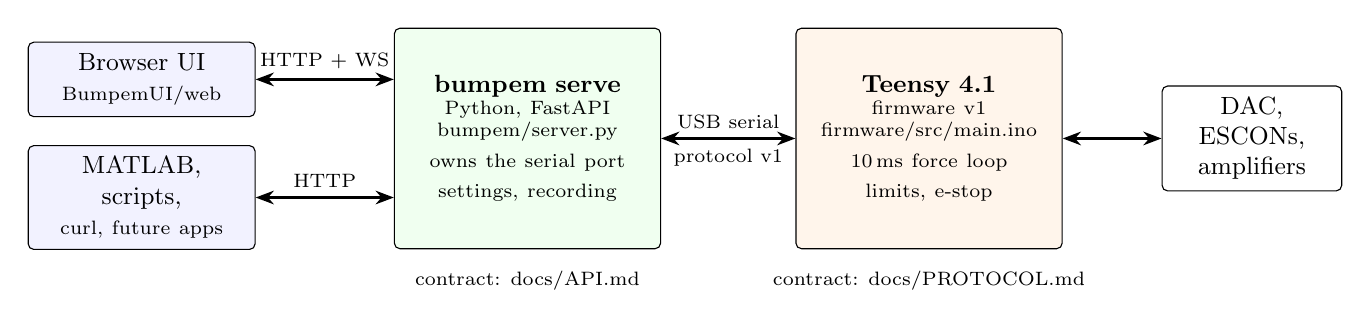
\begin{tikzpicture}[
  box/.style={draw, rounded corners=2pt, align=center, font=\small, inner sep=4pt},
  arr/.style={{Stealth}-{Stealth}, thick},
  lab/.style={font=\scriptsize, align=center}]
  \node[box, fill=blue!5, text width=2.6cm] (ui) at (0,0.75) {Browser UI\\\scriptsize BumpemUI/web};
  \node[box, fill=blue!5, text width=2.6cm] (other) at (0,-0.75) {MATLAB, scripts,\\\scriptsize curl, future apps};
  \node[box, fill=green!6, text width=3.1cm, minimum height=2.8cm] (srv) at (4.9,0) {\textbf{bumpem serve}\\\scriptsize Python, FastAPI\\\scriptsize bumpem/server.py\\[3pt]\scriptsize owns the serial port\\\scriptsize settings, recording};
  \node[box, fill=orange!8, text width=3.1cm, minimum height=2.8cm] (fw) at (10.0,0) {\textbf{Teensy 4.1}\\\scriptsize firmware v1\\\scriptsize firmware/src/main.ino\\[3pt]\scriptsize 10\,ms force loop\\\scriptsize limits, e-stop};
  \node[box, text width=2.0cm] (hw) at (14.1,0) {DAC, ESCONs, amplifiers};
  \draw[arr] (ui.east) -- node[lab, above]{HTTP + WS} (ui.east -| srv.west);
  \draw[arr] (other.east) -- node[lab, above]{HTTP} (other.east -| srv.west);
  \draw[arr] (srv) -- node[lab, above]{USB serial} node[lab, below]{protocol v1} (fw);
  \draw[arr] (fw) -- (hw);
  \node[lab, below=0.15cm of srv] {contract: docs/API.md};
  \node[lab, below=0.15cm of fw] {contract: docs/PROTOCOL.md};
\end{tikzpicture}
\caption{Software layers. Each arrow has one written contract; change the contract first, then the code
on both sides.}
\end{figure}

Why this split (\file{docs/DECISIONS.md} D6, D9, D10):
\begin{itemize}
\item The \textbf{Teensy} does all real-time work and all safety limits (force clamp, over-force fault,
e-stop, watchdog). It knows channels, forces and times, nothing about angles or gait.
\item The \textbf{server} is the only program that opens the serial port, so the stop command can never be
blocked by another program (the old MATLAB + serial monitor setup had exactly that problem). It turns
angles into per-module forces and will schedule gait-triggered perturbations.
\item The \textbf{UI} is replaceable. It uses only the HTTP API, never the Python code. Closing the browser
changes nothing on the board.
\item Everything runs without hardware: \file{bumpem/sim.py} is a simulated board that speaks the same
protocol. Use it first for every change.
\end{itemize}

\subsection{Firmware v1}\label{sec:firmware}
Built and flashed with PlatformIO: \file{scripts/flash.sh} (settings and pinned library versions in
\file{firmware/platformio.ini}). The original thesis code stays untouched in \file{legacy/};
\file{scripts/flash.sh} \cmd{legacy} builds it as a reference. Confirm with the project lead before flashing.

\paragraph{States.} \cmd{DISARMED} at boot (drivers off, no tension) $\rightarrow$ \cmd{ARM} ramps 0 to
baseline over \cmd{arm\_ms} $\rightarrow$ \cmd{ARMED} (holding baseline, pulses allowed) $\rightarrow$
\cmd{RELEASE} ramps to 0, drivers off. Any state $\rightarrow$ \cmd{ESTOP} (drivers off, DAC 0 at once;
recover with \cmd{ARM}). Measured force above \cmd{fault\_n} for \cmd{fault\_ms} $\rightarrow$ \cmd{FAULT}.

\paragraph{Control law} (per enabled module, every \cmd{loop\_ms}):
\[
i_\mathrm{des} = k_p\,(F_\mathrm{target}-F) - k_d\,\frac{\Delta F}{\Delta t}
  + k_\mathrm{ff}\,F_\mathrm{target}\,\frac{r_c}{k_t},\qquad
\mathrm{DAC} = \mathrm{clamp}\!\left(\frac{i_\mathrm{des}}{i_\mathrm{full}},0,1\right)\cdot 4095
\]
With $k_p = k_d = 0$ the loop is open: the motor gets a current proportional to the target and the force
sensor is ignored. ``Armed'' does not mean ``closed loop''; the gains decide.

\begin{table}[H]\centering\small
\begin{tabularx}{\linewidth}{lllX}
\toprule
Parameter & Default & Used on 6 Oct & Meaning \\
\midrule
\cmd{kp\_track}, \cmd{kd\_track} & 0.24, 3.5 & default & PD gains while holding baseline \\
\cmd{kp\_pulse}, \cmd{kd\_pulse} & 0.24, 3.5 & default & PD gains during a pulse \\
\cmd{kff} & 7.5 & 2 & feedforward multiplier (Stanford: 1) \\
\cmd{rc}, \cmd{kt} & 0.01905, 0.1524 & default & drum radius (m), torque constant \\
\cmd{i\_full} & 30 & default & current at DAC full scale (real: 9.9\,A, Sect.~2) \\
\cmd{baseline\_n} & 5 & 2 & holding tension, N \\
\cmd{fmax\_n} & 200 & 40 & largest allowed target, N (hard ceiling 200) \\
\cmd{fault\_n}, \cmd{fault\_ms} & 195, 20 & default & over-force fault \\
\cmd{filter\_hz}, \cmd{d\_window} & 0, 1 & default & force filter (0 = off), derivative window \\
\cmd{ch\_A}\ldots\cmd{ch\_D} & 1,1,1,0 & set by server & module enabled \\
\cmd{gain\_X}, \cmd{offset\_X} & 1, 0 & offsets zeroed & per-sensor calibration \\
\cmd{wd\_ms} & 0 & 1000 (server) & watchdog: no message for this long $\rightarrow$ abort pulse \\
\bottomrule
\end{tabularx}
\caption{Main parameters (full list in \file{docs/PROTOCOL.md}). They live in the Teensy's RAM: a replug
resets them, which is why the server reapplies saved settings.}
\end{table}

\paragraph{Serial protocol.} One text line per message. Host $\rightarrow$ board: \cmd{INFO}, \cmd{GET},
\cmd{SET name value}, \cmd{ARM}, \cmd{PULSE id delay rise dur fall aA aB aC aD}, \cmd{ABORT},
\cmd{RELEASE}, \cmd{ESTOP}, \cmd{CLEAR}, \cmd{STATS}, \cmd{PING}. Every command gets one \cmd{A,OK} or
\cmd{A,ERR} line. Board $\rightarrow$ host: telemetry \cmd{T,ms,state,pulse\_id,} then target, measured and
DAC value for A--D, 100 lines/s; events \cmd{E,...} (pulse start/end, state changes, faults).
Pulse amplitudes are relative to baseline; duration runs from start to end including both ramps.

\subsection{Python package and server}
Install once (conda env \cmd{BumpemHome} on the lab Mac):
\begin{lstlisting}
cd BumpemServer
pip install -e ".[server,dev]"
pytest                      # 52 tests, no hardware needed
\end{lstlisting}

\begin{table}[H]\centering\small
\begin{tabularx}{\linewidth}{lX}
\toprule
Module & Role \\
\midrule
\file{protocol.py} & message types and parser; mirrors \file{docs/PROTOCOL.md} \\
\file{device.py} & \cmd{Board} client: request/ack, telemetry, e-stop, over a serial link or the simulator \\
\file{sim.py} & simulated board speaking protocol v1 \\
\file{server.py} & HTTP/WebSocket server (FastAPI) \\
\file{geometry.py} & angle $\rightarrow$ per-module amplitudes \\
\file{datalog.py} & CSV recordings \\
\file{cli.py} & the \cmd{bumpem} command \\
\file{gait.py}, \file{experiment.py}, \file{recovery.py}, \file{vicon.py} & foot-strike detection (port of the MATLAB script, not yet validated), trial sequences, balance-recovery hook, Vicon client (stub) \\
\bottomrule
\end{tabularx}
\end{table}

\paragraph{Starting the server.}
\begin{lstlisting}
bumpem serve --board /dev/cu.usbmodem169222501 --modules ACD   # production (default)
bumpem serve --testing --board /dev/cu.usbmodem169222501       # one test pull per motor
bumpem serve --board sim                                        # no hardware
\end{lstlisting}
Then open \url{http://127.0.0.1:8000/} (UI) or \url{http://127.0.0.1:8000/docs} (try every endpoint).
Options: \cmd{--modules} (mounted modules; use \cmd{ABCD} once tower B runs), \cmd{--settings}
(default \file{settings.json}), \cmd{--log-dir} (default \file{Logs/}), \cmd{--wd-ms} (board watchdog,
default 1000), \cmd{--host} (default 127.0.0.1, this PC only), \cmd{--ui}.

\begin{table}[H]\centering\small
\begin{tabularx}{\linewidth}{llX}
\toprule
Method & Path (\cmd{/api/v1/...}) & Does \\
\midrule
GET/POST & \cmd{info}, \cmd{ports}, \cmd{connect}, \cmd{disconnect} & connection (\cmd{\{"port":"sim"\}} for the simulator) \\
GET/PATCH & \cmd{status}, \cmd{params} & board state, read/change parameters \\
POST & \cmd{arm}, \cmd{release}, \cmd{abort}, \cmd{estop}, \cmd{clear} & state changes \\
POST & \cmd{pulse} & one pulse, amplitudes per module \\
POST & \cmd{perturbation} & one pulse by angle + resultant amplitude \\
GET & \cmd{geometry} & module angles, reachable directions \\
GET/POST/DELETE & \cmd{settings} & saved parameters, reapplied at every connect \\
GET/POST & \cmd{log}, \cmd{log/start}, \cmd{log/stop} & recording to \file{Logs/force_*.csv} + \file{events_*.csv} \\
POST & \cmd{test/pull} & testing mode only: one open-loop pull on one module \\
WS & \cmd{stream} & live telemetry (30\,Hz for display) and events; accepts \cmd{\{"type":"estop"\}} \\
\bottomrule
\end{tabularx}
\caption{Implemented endpoints (\file{docs/API.md}). Errors come back as
\cmd{\{"error":\{"code":...,"message":...\}\}}; \cmd{board\_lost} (503) means the USB link is gone: replug,
then Disconnect and Connect.}
\end{table}

Example from MATLAB:
\begin{lstlisting}
opts = weboptions('MediaType', 'application/json');
webwrite('http://127.0.0.1:8000/api/v1/perturbation', struct('angle_deg', 135, ...
         'amplitude_n', 20, 'phase1_ms', 50, 'dur_ms', 400, 'phase2_ms', 50), opts);
\end{lstlisting}

\subsection{Browser UI}
Plain HTML, CSS and JavaScript in \file{BumpemUI/web}, no build step, works offline. The server serves it
at \cmd{/ui/}. Two pages, matching the server mode:
\begin{itemize}
\item \textbf{Testing} (\file{testing.html}, \cmd{--testing}): per motor a force and a duration, then
\emph{Pull}. No arming, no constant tension. Use it to check that each rope moves after any wiring change.
\item \textbf{Production} (\file{index.html}, default): Connect, Arm, Release, Clear; direction dial
(grey = no mounted module can pull that way); perturbation amplitude, ramps, duration, delay with a profile
preview; board settings (baseline, max force, feedforward gain, channels); \emph{Zero sensors} (2\,s mean
$\rightarrow$ offsets, ropes slack); \emph{Save as default}; \emph{Record} with a label; live force plot
(measured solid, target dashed); gait-phase picker (disabled until the server has PTO).
\end{itemize}
\textbf{STOP} (red button or the Esc key) is on every page. STOP and Release drop rope tension: stop the
treadmill first unless it is an emergency.

\begin{figure}[H]\centering
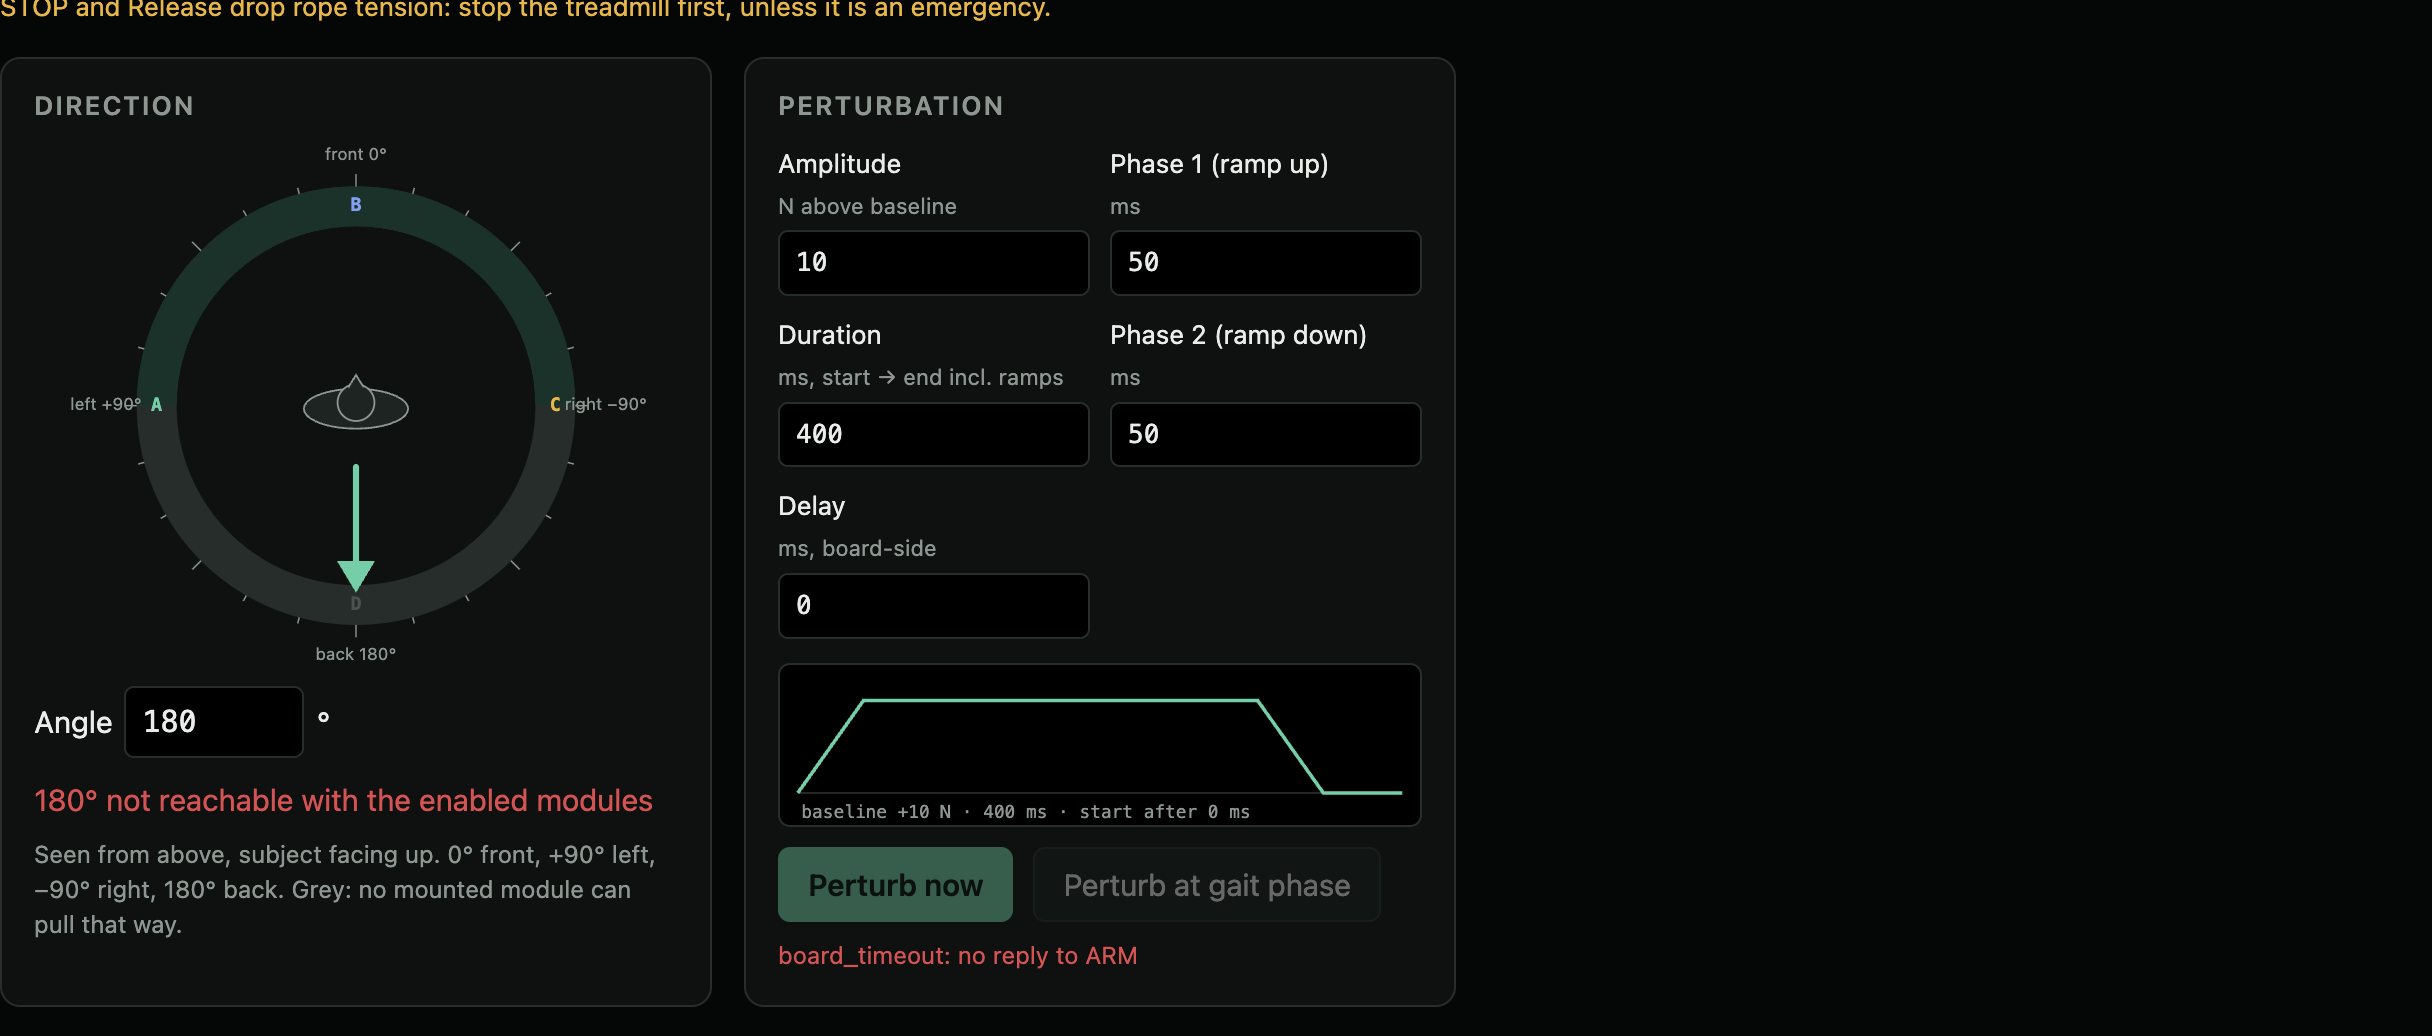
\includegraphics[width=\linewidth]{figures/ui-production.png}
\caption{Production page, 5 Oct 2026, B not installed so the front half of the dial is grey. The red
timeout under the button was the faulty USB socket, solved on 6 Oct.}
\end{figure}

\subsection{Not built yet}
\begin{enumerate}
\item \textbf{PTO}: perturb a set time or gait-cycle percentage after a foot strike (needs gait events,
first replayed, then from Vicon).
\item \textbf{Trials}: blocks, shuffled directions, 50--75 steps between perturbations, baseline from the
first 3\,s, logs. The schema is already proposed in \file{docs/API.md} (\cmd{planned}).
\item \textbf{Vicon live} on the lab PC (DataStream SDK) and the lab's balance-recovery algorithm
(\file{bumpem/recovery.py}, search \cmd{TODO(recovery)}).
\item Validate \file{bumpem/gait.py} against a recorded MATLAB log before live use.
\end{enumerate}

\subsection{How to change things}
\begin{itemize}
\item \textbf{New firmware behaviour}: \file{docs/PROTOCOL.md} first, then \file{firmware/src/main.ino},
then \file{bumpem/protocol.py} and \file{sim.py}. Re-flash.
\item \textbf{New endpoint}: \file{docs/API.md} first, then \file{server.py} + a test in
\file{tests/test_server.py}, then the UI.
\item \textbf{UI only}: edit \file{BumpemUI/web}, reload the page; test against \cmd{--board sim}.
\item After any change: \cmd{pytest}, update \file{docs/STATUS.md}, add a decision to
\file{docs/DECISIONS.md} if you chose between options, commit as \cmd{<area>: <what>}.
\end{itemize}

\section{Procedures}

\subsection{Power order}
\begin{description}
\item[Up] Teensy USB (boots DISARMED) $\rightarrow$ 24\,V (amplifiers) $\rightarrow$ check the force readings
$\rightarrow$ 48\,V $\rightarrow$ Arm.
\item[Down] Treadmill stopped $\rightarrow$ Release (or STOP) $\rightarrow$ 48\,V off $\rightarrow$ 24\,V off
$\rightarrow$ USB.
\end{description}
24\,V must come before 48\,V: without the amplifiers the Teensy reads 0\,N and the closed loop keeps raising
the current.

\subsection{Testing after any wiring change}
\begin{enumerate}
\item 48\,V off. Meter: continuity of each wire end to end; no continuity between 3.3\,V and GND.
\item USB only: \cmd{bumpem monitor --port PORT} shows 100 telemetry lines per second; \cmd{bumpem info}
answers.
\item \cmd{bumpem serve --testing ...}, testing page, 48\,V on, one module at a time: Pull 5\,N then 10\,N,
400--500\,ms. Only that module's rope moves.
\item With 24\,V on and ropes slack: each module reads a few N; pulling a rope by hand moves only its own
reading (\file{scripts/force_check.py}).
\end{enumerate}

\subsection{Closed loop}
\begin{enumerate}
\item Production page, connect, ropes slack: \emph{Zero sensors}.
\item Set a low feedforward (e.g.\ \cmd{kff} 2) and baseline 2\,N, \cmd{fmax\_n} 40, then \emph{Save as
default} so a replug keeps them.
\item Nobody in the harness. Arm one module at a time; it should hold 2--5\,N.
\item \emph{Record}, then perturbations of 10\,N, then 20\,N. Compare target and measured in the CSV.
Reference values from the thesis: 100\,N target $\rightarrow$ peak 96.7 $\pm$ 12.3\,N, rise time (to 80\,\%)
36 $\pm$ 5\,ms (\file{docs/knowledge/results.md}).
\end{enumerate}

\subsection{Configuring an ESCON}\label{sec:escon}
Configuration is done once per driver with ESCON Studio (Windows, USB on J7). No setting by hand.
\begin{enumerate}
\item Enable wire (J5 pin 2) unplugged, rope slack or off the drum, nobody near the tower.
\item USB in first, then 48\,V on. Open ESCON Studio; the controller appears.
\item Load a parameter file from \file{escon/} (module A's is the reference: current mode, enable on
DigIN2, setpoint on AnIN2, 0--10\,V = 0--30\,A). \emph{Download parameters} writes it into the
controller.
\item \emph{Regulation Tuning} (auto-tuning) with the motor free to turn: adapts the gains to that motor.
\item \emph{Store Parameters}, otherwise the driver forgets everything at power-off. Power-cycle and check
the values in the Controller Monitor.
\item Save the result as \file{escon/module<X>_<side>_<date>.edc} and commit it.
\item LED: slow green blink = ready (disabled). Red = error; count the flashes and look them up in
\file{escon/README.md}.
\item 48\,V off first, then USB out. Plug the enable wire back in.
\end{enumerate}
If ESCON Studio offers a firmware update, do not accept it without checking first.

\subsection{Calibrating a load cell}\label{sec:calibration}
Hang 6, 8 and 12\,kg (58.9, 78.5, 117.7\,N). First check with a meter that the amplifier output stays
$\leq$ 3.3\,V at the hardest pull (IAA100 DIP switches and zero/span pots). Small errors are corrected in
software with \cmd{gain\_X} and \cmd{offset\_X}; save them with \emph{Save as default}.

\subsection{Safety rules}
\begin{itemize}
\item The GRAIL treadmill e-stop stays the primary stop. Stop the treadmill \emph{before} Release or STOP:
both drop the rope tension.
\item First tests on any module: nobody attached, hand on the power strip switch.
\item Breakaway line on every rope; overhead fall-arrest harness for the subject.
\item No person in the harness until the e-stop is wired and tested.
\end{itemize}

\section{Faults found and what they teach}\label{sec:lessons}
Every fault below cost hours. Most were wiring, none were software. Check these first.

{\small
\begin{longtable}{>{\raggedright}p{3.6cm} >{\raggedright}p{5.4cm} >{\raggedright\arraybackslash}p{5.6cm}}
\toprule
Symptom & Cause & Lesson \\
\midrule\endhead
\bottomrule\endfoot
Module C: ESCON red LED, ``Hall sensor pattern error'' & Hall GND (blue) on J2 pin 4 (shield) instead of J3 pin 5. Same on a second module & Check J2/J3 colours against the table in Sect.~3 on every module. ESCON Studio's Diagnostics finds it. \\
Module A pulled far too hard & J3 green and grey swapped (Hall supply on a Hall input) & Same check. Run Diagnostics before the first drive. \\
Module D pulled far too hard at 2--5\,N & its green SP$-$ wire was on the 3.3\,V rail instead of GND & Breadboard rails are easy to confuse; the carrier board removes this. \\
Module A did nothing & loose breadboard contact & Reseat; carrier board. \\
C and D both on pin 17 & wiring error & One force pin per module (14--17). \\
Module C reads $\approx$ 73\,N at rest & white ground wire cut & A floating ground gives a large false force; never arm a module whose rest reading is not a few N. \\
``No reply'' timeouts at random & bad USB hub socket / cable; the link dropped even with 48\,V and 24\,V off & Check \cmd{bumpem monitor} gives 100 lines/s before suspecting software. Use the good socket. \\
Tower B broken & old 48\,V supply faulty (white residue); chopper at 75\,V instead of 55\,V & Check the chopper DIP on every tower. \\
Tower B: enable ignored, USB not seen & ESCON control side faulty (power stage passed meter tests) & Swap test: A's ESCON worked on the same PC and cable. \\
Closed loop held $\approx$ 15\,N instead of 2\,N after a replug & parameters reset to firmware defaults (kff 7.5, baseline 5, no offsets) & Fixed: the server reapplies \file{settings.json} at every connect. \\
\end{longtable}
}

\subsection{Open decisions}
\begin{itemize}
\item \cmd{i\_full} 9.9 (real ESCON scaling) and \cmd{kt} 0.231 (datasheet), after reading the configs of
C and D and the closed-loop tests.
\item Firmware boots with \cmd{ch\_D} = 0; the server switches it on. Changing the default needs a protocol
update and a re-flash.
\item Ropes are worn: choose a low-stretch rope with the breakaway as the weakest link.
\item Fail-safe e-stop (needs extra hardware).
\end{itemize}


\appendix
\section{Where to find things}

Repositories: \file{BumpemServer} (firmware, server, docs, hardware) and \file{BumpemUI} (web UI), side by
side in one folder. Large reference files are kept on disk only, not in git: ask the project lead for
\file{docs/thesis/}, \file{docs/reference/}, \file{docs/hardware-photos/} and \file{legacy/}.

{\small
\begin{longtable}{>{\raggedright}p{6.2cm} >{\raggedright\arraybackslash}p{8.6cm}}
\toprule
Path (in \file{BumpemServer} unless noted) & Contents \\
\midrule\endhead
\bottomrule\endfoot
\file{docs/STATUS.md}, \file{docs/TODO.md} & current state, day-to-day checklist \\
\file{docs/DECISIONS.md} & every design choice with its reason (D1, D2, \ldots) \\
\file{docs/FILES.md} & full file index \\
\file{docs/knowledge/} & facts extracted from thesis, manual and Stanford guide, with sources: hardware, wiring, control, calibration, safety, gait detection \\
\file{docs/PROTOCOL.md} & serial protocol, all firmware parameters \\
\file{docs/API.md} & server API \\
\file{docs/tests/} & meter test sheets (module C power checks, broken tower diagnosis) \\
\file{docs/power-estop-checklist.md} & power and e-stop checklist \\
\file{docs/parts-list.xlsx}, \file{docs/parts-to-buy.xlsx} & parts with prices and links \\
\file{escon/} & ESCON pin table, LED codes, parameter files (\file{.edc}) \\
\file{hardware/carrier/} & carrier PCB: generator scripts, KiCad project, gerbers, BOM \\
\file{hardware/enclosures/} & printed tower parts: CadQuery sources, STL/STEP, overview PDF \\
\file{firmware/} & Teensy firmware v1 (PlatformIO) \\
\file{bumpem/}, \file{tests/} & Python package and tests \\
\file{scripts/} & \file{flash.sh}, \file{open_loop_test.sh}, \file{force_check.py} \\
\file{legacy/} & original Arduino sketch and MATLAB script (read only) \\
\file{BumpemUI/web/} & UI pages \\
\file{docs/handbook/} & this document (LaTeX) \\
\end{longtable}
}

\subsection*{Contacts}
\begin{itemize}
\item HS Offenburg makerspace (carrier PCB): Sebastian Stulz.
\item maxon Germany (ESCON, chopper): info.de@maxongroup.com.
\item Mains wiring of the supplies: university electrician.
\end{itemize}


\end{document}
